\documentclass[11pt,a4paper]{article}

% Packages
\usepackage[utf8]{inputenc}
\usepackage[T1]{fontenc}
\usepackage{lmodern}
\usepackage[english,bahasai]{babel}
\usepackage[a4paper,margin=2.5cm]{geometry}
\usepackage{setspace}
\usepackage{graphicx}
\usepackage{booktabs}
\usepackage{tabularx}
\usepackage{longtable}
\usepackage{array}
\usepackage{amsmath}
\usepackage{float}
\usepackage{caption}
\usepackage{enumitem}
\usepackage{titlesec}
\usepackage{tocloft}
\usepackage[autostyle=false,style=english]{csquotes}
\usepackage[style=ieee,backend=biber,dashed=false]{biblatex}
\DeclareLanguageMapping{bahasai}{english}
\DefineBibliographyStrings{bahasai}{url = {\mkbibbrackets{Online}\adddot\addspace Available}, urlseen = {Accessed}}
\usepackage[hidelinks]{hyperref}

\addbibresource{../references.bib}
\graphicspath{{figures/}}
\setstretch{1.2}
\captionsetup{font=small,labelfont=bf}
\setlist{itemsep=2pt,topsep=4pt}

% Section Style (dokumen kajian kebijakan)
\renewcommand{\thesection}{\Roman{section}}
\renewcommand{\thesubsection}{\arabic{section}.\arabic{subsection}}
\titleformat{\section}{\normalfont\large\bfseries}{\thesection.}{0.6em}{\MakeUppercase}
\titleformat{\subsection}{\normalfont\normalsize\bfseries}{\thesubsection}{0.6em}{}
\setlength{\cftsecnumwidth}{2.6em}
\setlength{\cftsubsecnumwidth}{2.4em}
\renewcommand{\cftsecfont}{\bfseries}

% Document Info
\newcommand{\judul}{Integrasi PLTS Atap dan\\Pensiun Dini PLTU Batu Bara}
\newcommand{\subjudul}{Program Pasangan Kuota PLTS Atap dan Pensiun Dini PLTU IPP\\untuk Transisi Energi Berkeadilan di Sistem Jawa-Bali 2026-2040}
\newcommand{\sumber}[1]{\par\smallskip{\footnotesize Sumber: #1}}
\newcolumntype{L}[1]{>{\raggedright\arraybackslash}p{#1}}
\newcolumntype{Y}{>{\raggedright\arraybackslash}X}

\begin{document}

\pagenumbering{gobble}
\begin{titlepage}
\centering
{\normalsize TUGAS MATA KULIAH\par}
{\normalsize MK4066 Perubahan Iklim (Layanan)\par}
\vspace{0.6cm}
{\Large\bfseries DOKUMEN KAJIAN KEBIJAKAN\par}
\vspace{0.4cm}
{\LARGE\bfseries \judul\par}
\vspace{0.3cm}
{\normalsize \subjudul\par}
\vspace{0.6cm}

\includegraphics[width=3.2cm]{logo_itb}\par
\vspace{0.4cm}
{\small Dosen Pengampu:\par}
{\small Dr.rer.nat. Armi Susandi, M.T.\par}
\vspace{0.4cm}
{\small Disusun oleh Kelompok 17:\par}
\vspace{0.15cm}
{\scriptsize
\begin{tabular}{l l @{\hspace{1.2cm}} l l}
10124084 & Azzahra Rizqi Saffa & 15024052 & Alzena Atha Audya \\
10524012 & Danica Giovanni & 15024071 & Lidya Savarani Tarigan \\
10524057 & Nayma Feby Nur Safitri & 15124027 & Jessica Aulia Cahyana \\
10623042 & Pande I Made Niko Mevano W P & 15124032 & Qabil Radhiqa Handoyo \\
12023096 & Dimas Rayhan & 15124066 & Angga Setiawan \\
12225128 & Franzeska Jessica Mattea & 15325014 & Elja Manuella Joesta Damanik \\
12324059 & Fahri Masis Nurhidayat & 15325021 & Muhammad Rafi Hikaru Rahman \\
13123086 & Ananda Ghibran Fadlilah & 15325093 & Alya Gita Khairani \\
13123129 & Muhammad Azhar Shiddiq & 15524057 & Haidar Islama Muhammad Firdaus \\
13224028 & Isnaya Zalfa Kamila & 18023017 & Raynee Soe Putra \\
13424036 & Magdalena Conny H.C.L.T & 18124013 & Kayla Olivia Putri \\
13523144 & Muhamad Nazih Najmudin & 18224076 & Bram Sebastian Pangaribuan \\
\end{tabular}

}
\vspace{0.4cm}

{\small Ditujukan kepada:\par}
{\small Menteri Energi dan Sumber Daya Mineral, Menteri Keuangan,\\
Direktur Utama PT PLN (Persero), serta Satuan Tugas Transisi Energi\par}
\vfill
{\large\bfseries INSTITUT TEKNOLOGI BANDUNG\par}
{\normalsize BANDUNG\par}
{\normalsize 2026\par}
\end{titlepage}


\pagenumbering{roman}
\tableofcontents
\clearpage
\section*{Ringkasan}
\addcontentsline{toc}{section}{Ringkasan}

Sistem listrik Jawa-Bali menyerap 69,5\% penjualan listrik nasional \cite{D-PLN-STAT-2025} dan masih bertumpu pada 57 unit PLTU batu bara terhubung jaringan PLN dengan kapasitas 30,8 GW dan emisi sekitar 169 juta ton CO$_2$ per tahun \cite{D-GEM-GCPT}. Laporan Kelompok 17 memilih integrasi PLTS atap dan pensiun dini PLTU sebagai solusi transisi \cite{L-LAPORAN-K17}. PLTU dipensiunkan bertahap, kapasitasnya digantikan PLTS atap, beban investasi disebar melalui insentif dan kewajiban pemasangan, dan pekerja terdampak dilindungi.

Masalahnya bukan ketiadaan aturan. Kebijakan PLTS atap dan pensiun dini berjalan terpisah, sehingga PLTS atap dipandang PLN sebagai pengurang pendapatan, sedangkan pensiun dini dipandang sebagai beban kompensasi. Pembatalan pensiun dini Cirebon-1 pada Desember 2025 menunjukkan bahwa tanpa hitungan yang jelas tentang siapa menanggung apa, pensiun dini mudah ditunda \cite{B-BISNIS-CIREBON-BATAL-2025}.

Dokumen kajian ini merekomendasikan \textbf{program pasangan kuota PLTS atap dan pensiun dini PLTU IPP}. Setiap PLTU yang dipensiunkan dipasangkan dengan tambahan PLTS atap paling sedikit setara dayanya, didahului pengikatan dana luar, pembangkit pengganti, dan program bagi pekerja. Urutan pensiun mendahulukan PLTU milik IPP karena hanya pensiun PLTU IPP yang menghentikan pembayaran kapasitas oleh PLN. Seluruh penilaian dilakukan dengan platform terbuka PowerShift yang dikembangkan bersama kajian ini.

Simulasi roadmap Fase 1-3 di Jawa-Bali memensiunkan 3,0 GW PLTU IPP pada 2030-2035 dan menambah 3,19 GWp PLTS atap, atau 106\% dari daya yang dipensiunkan. Selama 2026-2040 paket ini menghindari 9.572 kematian dini dan 35,4 juta ton CO$_2$. Biaya bersih bagi negara Rp11,9 triliun, atau kurang dari Rp1 triliun per tahun, sementara pelanggan menghemat tagihan Rp38,0 triliun dan nilai kesehatan yang terselamatkan Rp111,3 triliun. Bila neraca negara harus nol, varian dengan PLTS atap lebih kecil menghasilkan surplus Rp1,8 triliun.

\begin{center}
\small
\begin{tabularx}{\textwidth}{*{4}{>{\centering\arraybackslash}X}}
\toprule
\textbf{3,0 GW} & \textbf{106\%} & \textbf{9.572 jiwa} & \textbf{Rp15,2 T} \\
PLTU IPP pensiun dini 2030-2035 & PLTS atap tambahan terhadap daya PLTU yang dipensiunkan & kematian dini dihindari 2026-2040 & dana luar, di bawah alokasi CIPP JETP sekitar Rp21,5 T \\
\bottomrule
\end{tabularx}
\end{center}

\clearpage
\pagenumbering{arabic}

\section{Pendahuluan: Konteks dan Urgensi}
\label{sec:pendahuluan}

\subsection{Latar Belakang}

Pemanasan global akibat aktivitas manusia meningkatkan risiko cuaca ekstrem, kekeringan, dan kenaikan muka laut \cite{P-IPCC-2023}. Di Indonesia, sektor ketenagalistrikan masih bertumpu pada PLTU batu bara. Sistem Jawa-Madura-Bali mengoperasikan 57 unit PLTU terhubung jaringan PLN dengan kapasitas 30,8 GW \cite{D-GEM-GCPT}. Emisinya juga membawa polutan udara yang menurut CREA dan IESR menyebabkan sekitar 10.500 kematian dini pada 2022 \cite{P-CREA-IESR-2023}.

Kerangka hukum untuk mengakhiri PLTU sudah tersedia melalui Perpres 112/2022 dan Permen ESDM 10/2025 \cite{R-PERPRES-112-2022,R-PERMEN-ESDM-10-2025}. CIPP JETP menargetkan pensiun dini 1,7 GW hingga 2040 \cite{P-JETP-CIPP-2023,P-CREA-CIPP-2023}. Di sisi energi bersih, pemerintah menetapkan kuota PLTS atap 2 GW hingga 2028, dengan 1,85 GW di Jawa-Madura-Bali \cite{B-CNBC-ROOFTOP-2028}. Realisasinya baru 538 MWp pada Juli 2025 \cite{B-KONTAN-ROOFTOP-2025}. Sementara itu, proyek percontohan pensiun dini Cirebon-1 dibatalkan pada Desember 2025 \cite{B-BISNIS-CIREBON-BATAL-2025,B-PETROMINDO-CIREBON-BATAL}.

Laporan Kelompok 17 menjawab situasi ini dengan memilih integrasi PLTS atap dan pensiun dini PLTU sebagai solusi \cite{L-LAPORAN-K17}. Solusi tersebut memuat empat mekanisme, yaitu penghentian PLTU bertahap, substitusi kapasitas melalui PLTS atap, penyebaran beban investasi melalui insentif dan kewajiban pemasangan, serta jaring pengaman sosial dan pelatihan ulang. Pelaksanaannya diatur dalam roadmap empat fase. Dokumen kajian ini menurunkan solusi tersebut menjadi program kebijakan yang dapat dihitung, dijalankan, dan dipantau.

\subsection{Rumusan Masalah}

\begin{enumerate}
  \item Mengapa PLTS atap dan pensiun dini PLTU belum berjalan bersamaan, dan celah kebijakan apa yang menyebabkannya?
  \item Bagaimana rancangan program yang memasangkan keduanya sehingga dapat diterima PLN dan negara?
  \item Seberapa layak program tersebut dari sisi fiskal, keandalan, kesehatan, dan sosial, serta bagaimana tahapan pelaksanaannya?
\end{enumerate}

\subsection{Tujuan dan Sasaran Pengguna}

Kajian ini bertujuan untuk (1) memetakan celah kebijakan yang memisahkan PLTS atap dan pensiun dini, (2) merumuskan program pasangan kuota PLTS atap dan pensiun dini beserta aturan pelaksanaannya, dan (3) menilai kelayakan serta menyusun langkah yang dapat langsung ditindaklanjuti.

Dokumen ini ditujukan kepada Kementerian ESDM sebagai penyusun regulasi dan kuota, Kementerian Keuangan sebagai pengelola insentif dan pendanaan, PT PLN (Persero) sebagai pelaksana kajian pensiun dini dan operator sistem, serta Satuan Tugas Transisi Energi yang diusulkan laporan kelompok sebagai koordinator lintas kementerian.

\subsection{Ruang Lingkup}

Kajian difokuskan pada sistem Jawa-Bali karena menampung sebagian besar PLTU dan penjualan listrik nasional. PLTU yang dikaji adalah unit operasi terhubung jaringan PLN, tidak termasuk PLTU captive industri. Horizon simulasi adalah 2026-2040, sejalan dengan target CIPP JETP. PLTS atap diperlakukan sebagai pengganti energi, bukan pengganti daya mampu saat beban puncak malam hari.

\subsection{Metode Kajian}

Kajian ini memakai analisis kebijakan berbasis bukti dalam empat langkah. Pertama, studi data sekunder dari Global Energy Monitor, Statistik PLN 2025, Global Solar Atlas, CREA dan IESR, serta regulasi dan pemberitaan 2022-2026. Kedua, analisis celah kebijakan dengan membandingkan regulasi yang berlaku terhadap kebutuhan solusi terpilih. Ketiga, simulasi tahunan 2026-2040 dengan model PowerShift yang menghitung neraca PLN, APBN, dana luar, keandalan, emisi, dan kematian dini terhadap baseline phase down di akhir kontrak. Keempat, penyusunan instrumen pelaksanaan berupa SOP, rancangan peraturan, dan lembar penilaian kandidat.

Angka dalam kajian ini mengutamakan sumber primer atau sumber yang dapat diperiksa ulang. Beberapa angka laporan kelompok dimutakhirkan dengan data yang lebih baru atau lebih rinci, misalnya kuota PLTS atap per wilayah dan kompensasi pensiun dini yang dikalibrasi ke nilai refinancing Cirebon-1. Daftar pemutakhiran tersebut dicantumkan pada Lampiran~\ref{lamp:pemutakhiran}.

\section{Definisi Masalah}
\label{sec:masalah}

\subsection{Beban PLTU yang Tidak Ditanggung Pengelolanya}

PLTU Jawa-Bali terkonsentrasi di Banten, Jawa Tengah, dan Jawa Timur, sedangkan dampaknya menyebar ke kawasan padat penduduk (Tabel~\ref{tab:pltu}). Sebanyak 18,8 GW dimiliki IPP dan 12,0 GW dimiliki PLN. Dampak kesehatan tidak merata antar-PLTU. Untuk Cirebon-1, CREA memperkirakan pensiun pada 2035 menghindari 6.370 kematian selama 2036-2042, atau sekitar 910 kematian per tahun \cite{B-ECOBUSINESS-CIREBON}. Biaya kesehatan ini tidak masuk ke harga listrik.

\begin{table}[H]
\centering
\caption{PLTU terhubung jaringan PLN Jawa-Bali per provinsi}
\label{tab:pltu}
\small
\begin{tabular}{lrrrrrr}
\toprule
Provinsi & Unit & MW & IPP (MW) & PLN (MW) & Mt CO$_2$/tahun & Kematian/tahun \\
\midrule
Banten & 19 & 10.527 & 4.642 & 5.885 & 57,6 & 2.723 \\
Jawa Tengah & 15 & 10.090 & 8.800 & 1.290 & 52,4 & 2.610 \\
Jawa Timur & 12 & 6.155 & 3.365 & 2.790 & 36,3 & 1.592 \\
Jawa Barat & 8 & 3.624 & 1.584 & 2.040 & 19,9 & 1.676 \\
Bali & 3 & 426 & 426 & 0 & 2,7 & 110 \\
\midrule
Total & 57 & 30.822 & 18.817 & 12.005 & 168,9 & 8.711 \\
\bottomrule
\end{tabular}

\sumber{Global Energy Monitor \cite{D-GEM-GCPT}. Kematian dini dari faktor rata-rata armada CREA \cite{P-CREA-IESR-2023}, kecuali Cirebon-1 \cite{B-ECOBUSINESS-CIREBON}}
\end{table}

\subsection{Kontrak dan Kompensasi Menghambat Pensiun Dini}

PLN membayar pembayaran kapasitas kepada IPP selama unit tersedia, terlepas dari listriknya dipakai atau tidak \cite{P-IEEFA-2017}. Mengakhiri kontrak lebih awal menimbulkan kewajiban kompensasi atas keuntungan yang hilang. Pensiun sebelum aset habis disusutkan juga menimbulkan risiko aset terdampar \cite{P-KEFFORD-2018}. Pada kasus Cirebon-1, ADB menyiapkan refinancing US\$250-300 juta untuk percepatan sekitar tujuh tahun \cite{B-REUTERS-CIREBON-2022,B-ADB-CIREBON}, sedangkan PLN menilai kewajibannya mencapai sekitar Rp60 triliun dan memilih pendekatan phase down \cite{B-PETROMINDO-CIREBON-BATAL,B-MONGABAY-202601}. Selisih penilaian sebesar ini menunjukkan bahwa besaran kompensasi adalah titik perdebatan utama.

\subsection{PLTS Atap Terhambat Aturan dan Modal Awal}

Permen ESDM 2/2024 menghapus perhitungan ekspor listrik sebagai pengurang tagihan dan menetapkan kuota per wilayah \cite{R-PERMEN-ESDM-2-2024}. Tanpa nilai ekspor, PLTS atap rumah tangga kurang menarik karena konsumsi rumah tangga tinggi pada malam hari, sehingga adopsi bergeser ke sektor komersial dan industri \cite{P-IESR-PERMEN2,B-PVMAG-QUOTA}. Harga pemasangan masih berada pada kisaran belasan juta rupiah per kWp \cite{B-DETIK-HARGA-PLTS}. Realisasi 538 MWp pada Juli 2025 masih jauh dari kuota 2 GW pada 2028 \cite{B-KONTAN-ROOFTOP-2025,B-CNBC-ROOFTOP-2028}.

\subsection{Beban Fiskal Berpindah ke APBN}

Tarif listrik ditetapkan pemerintah di bawah biaya pokok penyediaan (BPP). Subsidi listrik 2026 diusulkan Rp97,37-104,97 triliun untuk 44,88 juta pelanggan \cite{B-KONTAN-SUBSIDI-2026}. Setiap tambahan biaya PLN pada akhirnya berpindah ke APBN. Ketika PLTS atap mengurangi penjualan PLN, pendapatan PLN turun, sedangkan pembayaran kapasitas PLTU tetap berjalan. Kondisi inilah yang membuat PLN menolak nilai ekspor PLTS atap selama sistem Jawa-Bali kelebihan pasokan \cite{B-TENGGARA-2024}.

\subsection{Pekerja dan Daerah Terdampak}

Cirebon-1 mempekerjakan sekitar 300 orang. CELIOS memperkirakan sedikitnya 14.000 pekerja langsung dan tidak langsung terdampak bila Cirebon-1 dan Pelabuhan Ratu dipensiunkan \cite{B-ECOBUSINESS-CIREBON}. Sebaliknya, PLTS atap termasuk teknologi energi paling padat karya, sekitar 24,72 job-year per MW \cite{P-CEEW-2017}. Peluang ini tidak otomatis menyerap pekerja PLTU tanpa program pelatihan ulang yang dijadwalkan.

\section{Analisis Celah Kebijakan (Policy Gap)}
\label{sec:celah}

\subsection{Kerangka Regulasi yang Berlaku}

Tabel~\ref{tab:regulasi} membandingkan regulasi dan rencana yang berlaku dengan kebutuhan solusi terpilih.

\begin{table}[H]
\centering
\caption{Regulasi terkait dan celahnya terhadap solusi integrasi}
\label{tab:regulasi}
\small
\begin{tabularx}{\textwidth}{L{3.6cm} Y Y}
\toprule
Regulasi atau rencana & Yang diatur & Celah terhadap solusi integrasi \\
\midrule
Perpres 112/2022 \cite{R-PERPRES-112-2022} & Percepatan energi terbarukan, larangan PLTU baru, peta jalan pengakhiran PLTU & Peta jalan tidak menyebut sumber energi pengganti per PLTU \\
\addlinespace
Permen ESDM 10/2025 \cite{R-PERMEN-ESDM-10-2025} & Kriteria pensiun dini Pasal 11 dan kewajiban kajian oleh PLN & Kriteria belum menimbang jenis kontrak (IPP atau PLN) dan dampak kesehatan per lokasi. Hasil kajian PLN tidak dibuka \\
\addlinespace
Permen ESDM 2/2024 \cite{R-PERMEN-ESDM-2-2024} & PLTS atap terhubung jaringan, kuota per wilayah, ekspor tidak mengurangi tagihan & Kuota ditetapkan tanpa dikaitkan dengan PLTU yang akan dipensiunkan \\
\addlinespace
Kuota PLTS atap hingga 2028 \cite{B-CNBC-ROOFTOP-2028} & 2 GW nasional, 1,85 GW Jawa-Madura-Bali & Realisasi tertinggal, belum ada kewajiban bagi gedung pemerintah dan BUMN \\
\addlinespace
CIPP JETP \cite{P-JETP-CIPP-2023} & Target pensiun dini 1,7 GW hingga 2040 & Alokasi dana kecil dan tidak dipersyaratkan terikat sebelum penutupan \\
\addlinespace
RUPTL 2025-2034 \cite{B-LISTRIKID-RUPTL-JAMALI} & Tambahan pembangkit Jamali termasuk surya skala besar & Pembangkit pengganti tidak dijadwalkan terhadap tanggal penutupan PLTU tertentu \\
\bottomrule
\end{tabularx}
\end{table}

\subsection{Celah Kebijakan Kritis}

Berdasarkan perbandingan di atas, kajian ini mengidentifikasi enam celah yang saling berkaitan.

\begin{enumerate}
  \item \textbf{Celah keterpaduan.} PLTS atap dan pensiun dini diatur oleh dua peraturan yang tidak saling merujuk. Akibatnya, PLTS atap dihitung PLN sebagai pengurang pendapatan, bukan sebagai pengganti PLTU yang membuka penghematan.
  \item \textbf{Celah pemilihan PLTU.} Pensiun dini PLTU IPP menghentikan pembayaran kapasitas, sedangkan pensiun dini PLTU milik PLN tidak. Perbedaan ini menentukan apakah pensiun dini menguntungkan atau membebani negara (Bagian~\ref{sec:kelayakan}), tetapi belum menjadi pertimbangan eksplisit dalam kriteria.
  \item \textbf{Celah pendanaan.} Belum ada mekanisme yang memastikan kompensasi dari dana luar terikat sebelum keputusan penutupan. Pembatalan Cirebon-1 terjadi pada tahap ini.
  \item \textbf{Celah keandalan.} Reserve margin Jawa-Bali diperkirakan turun ke batas aman 33\% sekitar 2027-2029 \cite{B-PETROMINDO-RESERVE}. Setelah itu, setiap PLTU yang pensiun memerlukan pembangkit pengganti yang siap lebih dulu. PLTS atap tidak menambah daya mampu saat beban puncak malam hari.
  \item \textbf{Celah transisi berkeadilan.} Program pelatihan ulang belum dijadwalkan terhadap tanggal penutupan setiap PLTU.
  \item \textbf{Celah data dan transparansi.} Kajian pensiun dini PLN dan kontrak IPP tidak terbuka. Pemangku kepentingan tidak memiliki alat bersama untuk menguji siapa menanggung biaya dan manfaat suatu usulan, sehingga perbedaan penilaian seperti pada Cirebon-1 sulit diselesaikan.
\end{enumerate}

Keenam celah ini menunjukkan bahwa persoalannya bukan kekurangan teknologi. Yang belum ada adalah aturan yang memasangkan PLTS atap dengan pensiun dini, urutan pemilihan PLTU yang menguntungkan negara, syarat penutupan yang jelas, dan alat hitung bersama yang dapat dipercaya semua pihak.

\section{Rekomendasi Kebijakan: Program Pasangan Kuota PLTS Atap dan Pensiun Dini}
\label{sec:rekomendasi}

\subsection{Gambaran Program}

Untuk menjawab keenam celah pada Bab~\ref{sec:celah}, kajian ini merekomendasikan program pasangan kuota PLTS atap dan pensiun dini PLTU. Program ini menjabarkan solusi terpilih laporan kelompok menjadi aturan yang dapat dijalankan. Setiap PLTU yang dipensiunkan dipasangkan dengan tambahan PLTS atap paling sedikit setara dayanya, dan penutupan baru dilakukan setelah dana, pengganti, dan program pekerja siap.

Program ini berpegang pada lima prinsip:
\begin{enumerate}
  \item \textbf{Berpasangan}, yaitu kuota PLTS atap dihitung dari rencana pensiun dini, bukan ditetapkan terpisah.
  \item \textbf{Hemat bagi negara}, yaitu PLTU dipilih berdasarkan dampaknya terhadap neraca negara per GW, sehingga pensiun dini PLTU IPP didahulukan.
  \item \textbf{Bersyarat}, yaitu penutupan dilakukan hanya setelah dana luar terikat, pembangkit pengganti siap, dan pekerja tercakup program.
  \item \textbf{Berbagi beban}, yaitu investasi PLTS atap disebar ke APBN, BUMN, dan swasta melalui kewajiban dan insentif.
  \item \textbf{Terbuka}, yaitu setiap usulan dinilai dengan alat hitung yang sama dan dapat diperiksa ulang.
\end{enumerate}

\subsection{Komponen Program}

Program terdiri atas enam komponen. Setiap komponen menjawab satu atau lebih celah kebijakan (Tabel~\ref{tab:komponen}).

\begin{table}[H]
\centering
\caption{Komponen program pasangan kuota PLTS atap dan pensiun dini}
\label{tab:komponen}
\small
\begin{tabularx}{\textwidth}{L{0.7cm} L{3.3cm} Y L{1.9cm}}
\toprule
Kode & Komponen & Isi utama & Celah \\
\midrule
K1 & Kuota berpasangan & Kuota PLTS atap tahunan di suatu sistem paling sedikit sama dengan kapasitas PLTU yang dijadwalkan pensiun di sistem tersebut & 1 \\
\addlinespace
K2 & Kewajiban dan insentif PLTS atap & Mulai 2028, gedung pemerintah dan BUMN di Jawa-Bali wajib memasang 200 MW per tahun. Industri memperoleh insentif fiskal 15\% dari harga pemasangan & 1 \\
\addlinespace
K3 & Urutan pensiun dini & PLTU dipilih dari daftar urut neraca negara per GW. PLTU IPP berdampak kesehatan tinggi didahulukan, PLTU milik PLN ditunda ke Fase 4 & 2 \\
\addlinespace
K4 & Syarat penutupan & Dana luar paling sedikit 80\% kompensasi terikat dan pembangkit pengganti beroperasi sebelum tanggal penutupan & 3, 4 \\
\addlinespace
K5 & Transisi pekerja & Pelatihan ulang dan perlindungan sosial bagi pekerja PLTU dimulai paling lambat satu tahun sebelum penutupan, diarahkan ke pemasangan dan pemeliharaan PLTS atap & 5 \\
\addlinespace
K6 & Alat hitung bersama PowerShift & Platform terbuka untuk menyaring kandidat, menguji paket, dan memantau indikator roadmap dengan data dan rumus yang sama bagi semua pihak & 6 \\
\bottomrule
\end{tabularx}
\end{table}

\subsection{Mekanisme Pasangan dan Syarat Penutupan}

Komponen K1, K3, dan K4 membentuk mekanisme inti program. Untuk setiap PLTU yang diusulkan pensiun pada tahun $Y$, Satgas memeriksa empat syarat berikut.
\begin{enumerate}
  \item \textbf{Neraca negara per GW tidak negatif} pada penyaringan kandidat di PowerShift. Syarat ini memastikan pensiun dini tidak membebani APBN dalam horizon kajian.
  \item \textbf{Rencana tambahan PLTS atap} hingga akhir roadmap (2040) paling sedikit sama dengan seluruh kapasitas PLTU yang dipensiunkan, dengan lintasan tahunan yang dipantau. Selama PLTS atap masih tertinggal, kekurangannya ditutup pembangkit pengganti pada syarat keempat.
  \item \textbf{Dana luar terikat} paling sedikit 80\% dari kompensasi.
  \item \textbf{Pembangkit pengganti siap} sebesar kapasitas yang diperlukan agar reserve margin tetap 33\%.
\end{enumerate}

Sebagai ilustrasi, Cirebon-1 (660 MW, IPP) yang dipensiunkan pada 2030 memerlukan kompensasi sekitar Rp0,69 triliun per tahun percepatan dengan estimasi skema ETM, atau Rp7,6 triliun selama 2030-2040. Dengan 80\% dari dana luar, porsi PLN Rp1,5 triliun dan dana luar Rp6,1 triliun. Pada saat yang sama, PLN berhenti membayar kapasitas Cirebon-1. Bila dipensiunkan sendiri, Cirebon-1 memberi neraca negara positif Rp4,3 triliun, atau Rp6,5 triliun per GW, sehingga syarat pertama terpenuhi. Kewajiban dan insentif K2 menambah sekitar 680 MWp PLTS atap di atas baseline pada 2028-2030, sedikit di atas 660 MW, sehingga syarat kedua juga terpenuhi.

\subsection{Perlindungan Pekerja dan Rumah Tangga}

Laporan kelompok menekankan transisi berkeadilan \cite{L-LAPORAN-K17}. Kajian ini mengusulkan tiga ketentuan minimum. Pertama, daftar pekerja langsung setiap PLTU kandidat disusun saat kandidat ditetapkan, bersama pemerintah daerah. Kedua, pelatihan ulang dimulai paling lambat satu tahun sebelum penutupan dan diarahkan ke pekerjaan pemasangan dan pemeliharaan PLTS atap yang tumbuh dari K2. Ketiga, dampak tarif dipantau. Program dirancang agar kenaikan BPP tetap kecil, di bawah Rp6 per kWh pada roadmap, sehingga tidak perlu kenaikan tarif rumah tangga rentan.

\subsection{PowerShift sebagai Alat Bantu Program}

PowerShift adalah platform web terbuka yang dikembangkan bersama kajian ini sebagai komponen K6. Platform ini tidak menggantikan kajian resmi PLN, melainkan menyediakan perhitungan bersama yang dapat diperiksa semua pihak. Fungsinya dipetakan ke tahapan program sebagai berikut.
\begin{itemize}
  \item \textbf{Penyaringan kandidat} (tab Kandidat PLTU): setiap PLTU dihitung seolah dipensiunkan sendiri pada tahun pilihan, lalu diurutkan menurut neraca negara per GW. Hasilnya adalah daftar urut untuk syarat pertama.
  \item \textbf{Perakitan paket} (panel kebijakan dan peta): PLTU terpilih, tahun pensiun, kewajiban PLTS atap, insentif industri, dan porsi pendanaan diatur dalam satu skenario.
  \item \textbf{Pemeriksaan syarat dan indikator} (tab Indikator roadmap dan Kriteria Permen 10/2025): kesetaraan PLTS atap beserta grafik lintasan tahunannya, kuota 2028, pembangkit pengganti, dana luar, pekerja, dan kriteria Pasal 11 ditampilkan per skenario dan per fase.
  \item \textbf{Analisis biaya dan manfaat} (tab Neraca, Keandalan, Dampak): neraca PLN, APBN, dan negara per tahun, reserve margin, emisi, dan kematian dini.
  \item \textbf{Perbandingan dan uji ketahanan} (tab Analisis): skenario aktif dipecah menjadi komponen PLTS atap dan pensiun dini, dibandingkan dengan skenario roadmap lain, dan diuji sensitivitasnya terhadap perubahan parameter kunci $\pm$20\%.
  \item \textbf{Berbagi dan pemantauan}: skenario disimpan sebagai tautan dan diekspor ke CSV, sehingga usulan antarlembaga dapat dibandingkan dengan dasar yang sama.
\end{itemize}

\begin{figure}[H]
\centering
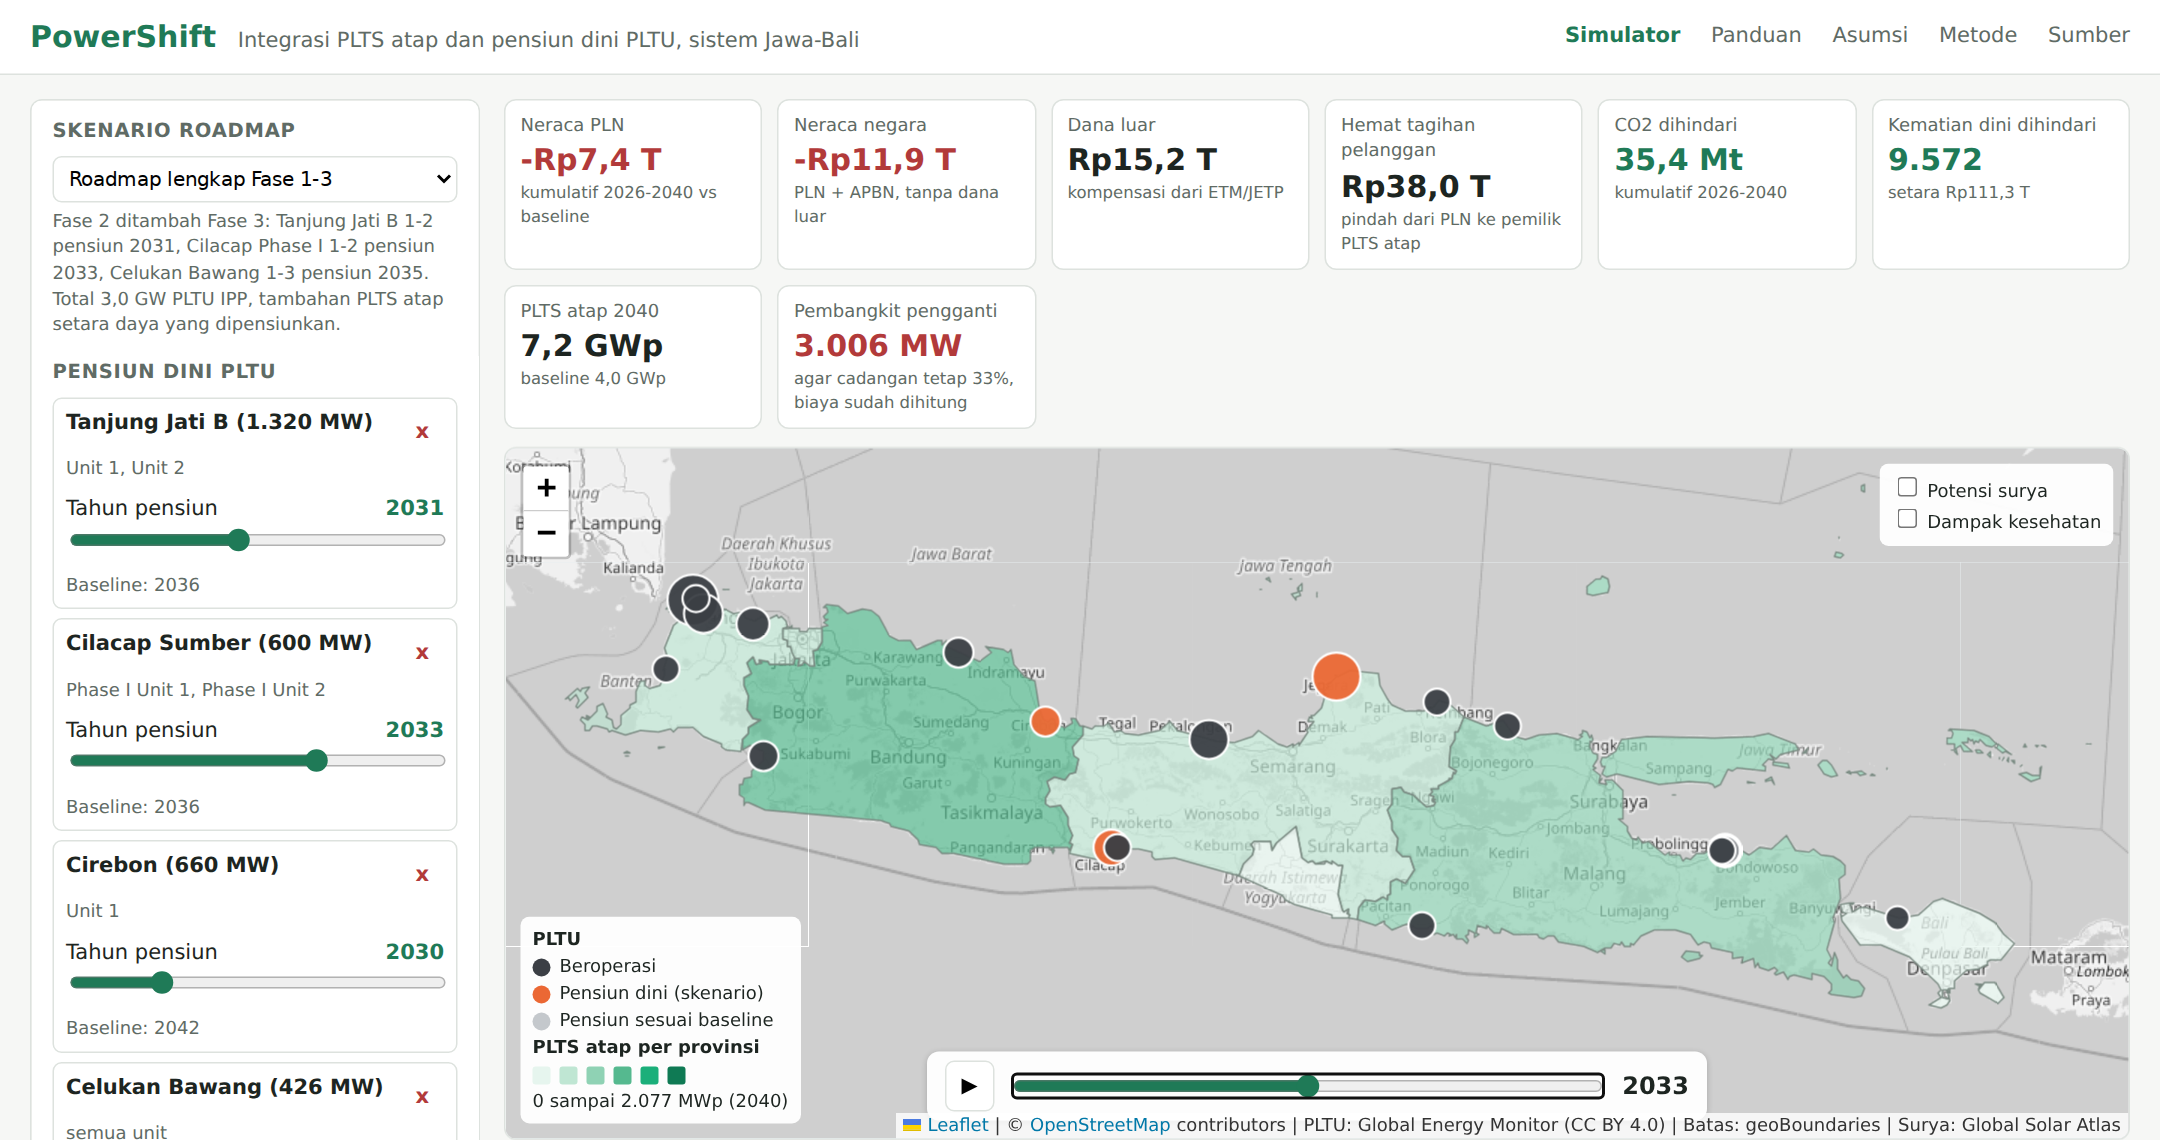
\includegraphics[width=\textwidth]{app_powershift}
\caption{Tampilan PowerShift pada skenario Roadmap Fase 1-3, tahun 2033}
\label{fig:app}
\sumber{\url{https://nazihnajmudin.github.io/Proyek-Periklim/}}
\end{figure}

\subsection{Kebaruan Program}

PLTS atap, pensiun dini, dan model neraca listrik masing-masing sudah dikenal. Kebaruan program ini terletak pada tiga hal. Pertama, kuota PLTS atap dikaitkan langsung dengan rencana pensiun dini sehingga PLTS atap dihitung sebagai pengganti. Kedua, urutan pensiun ditentukan oleh dampak terhadap neraca negara per GW, yang membedakan PLTU IPP dan PLTU milik PLN. Ketiga, seluruh penilaian dilakukan dengan alat terbuka yang memetakan biaya dan manfaat ke PLN, APBN, dana luar, pelanggan, dan kesehatan sekaligus.

\section{Analisis Kelayakan dan Proyeksi Dampak}
\label{sec:kelayakan}

\subsection{Asumsi Simulasi}

Simulasi memakai model tahunan PowerShift untuk 2026-2040. Baseline adalah phase down, yaitu PLTU IPP pensiun di akhir PPA, PLTU PLN pensiun di akhir umur desain, dan PLTS atap tumbuh mengikuti tren tanpa nilai ekspor. Asumsi utamanya adalah sebagai berikut. Seluruh parameter beserta sumber dan status verifikasinya tercantum pada Lampiran~\ref{lamp:asumsi}.
\begin{itemize}
  \item Produksi PLTS atap rata-rata 1.424 kWh/kWp/tahun, tertimbang penjualan listrik per provinsi \cite{D-GSA-PVOUT,D-PLN-STAT-2025}.
  \item Adopsi PLTS atap mengikuti kurva pangsa pasar terhadap waktu balik modal $\exp(-0{,}3 \times \text{payback})$ \cite{P-NREL-SOLARDS}, dibatasi kuota.
  \item Kompensasi pensiun dini PLTU IPP memakai estimasi skema ETM sebesar Rp1,045 miliar per MW per tahun percepatan, dikalibrasi ke refinancing Cirebon-1 US\$250-300 juta \cite{B-REUTERS-CIREBON-2022}. Untuk PLTU PLN, kompensasi berupa nilai buku yang hilang.
  \item Energi PLTU yang dipensiunkan digantikan PLTS atap tambahan dan sisa armada pada biaya marjinal batu bara DMO.
  \item Reserve margin dijaga 33\%. Kekurangan daya mampu dipenuhi pembangkit pengganti dengan biaya US\$120/kW/tahun.
  \item Nilai kesehatan US\$0,7 juta per kematian dini \cite{P-CREA-IESR-2023}.
\end{itemize}

\subsection{Penyaringan Kandidat Pensiun Dini}

Tabel~\ref{tab:kandidat} adalah keluaran tab Kandidat PLTU di PowerShift. Setiap PLTU dihitung seolah dipensiunkan sendiri pada 2031 dengan 80\% kompensasi dari dana luar.

\begin{table}[H]
\centering
\caption{Daftar urut kandidat pensiun dini 2031 menurut neraca negara per GW}
\label{tab:kandidat}
\resizebox{\textwidth}{!}{\begin{tabular}{rllrrrrrr}
\toprule
\# & PLTU & Pemilik & MW & Pensiun baseline & Neraca negara (Rp T) & Per GW (Rp T) & Dana luar (Rp T) & Kematian/tahun \\
\midrule
1 & Celukan Bawang & IPP & 426 & 2045 & 4,8 & 11,3 & 3,6 & 110 \\
2 & Paiton-3 & IPP & 815 & 2042 & 4,8 & 5,9 & 6,8 & 211 \\
3 & Cilacap Sumber & IPP & 2.260 & 2036 & 10,7 & 4,7 & 16,4 & 585 \\
4 & Tanjung Jati B & IPP & 4.640 & 2036 & 21,7 & 4,7 & 33,3 & 1.200 \\
5 & Cirebon & IPP & 1.584 & 2042 & 7,1 & 4,5 & 13,2 & 1.149 \\
6 & Serang & IPP & 660 & 2047 & 2,5 & 3,8 & 5,5 & 171 \\
7 & Jawa-7 & IPP & 1.982 & 2049 & 6,8 & 3,4 & 16,6 & 513 \\
8 & Batang (Central Java Power) & IPP & 1.900 & 2052 & 6,5 & 3,4 & 15,9 & 491 \\
9 & Paiton & PLN & 400 & 2033 & -0,8 & -2,0 & 0,7 & 103 \\
10 & Suralaya & PLN & 4.425 & 2036 & -14,9 & -3,4 & 25,9 & 1.144 \\
11 & Tanjung Awar-Awar & PLN & 700 & 2052 & -8,4 & -12,0 & 2,3 & 181 \\
12 & Pacitan & PLN & 630 & 2051 & -7,6 & -12,0 & 2,2 & 163 \\
13 & Rembang & PLN & 630 & 2051 & -7,6 & -12,0 & 2,2 & 163 \\
14 & Indramayu & PLN & 990 & 2050 & -11,9 & -12,0 & 3,5 & 256 \\
15 & Labuan & PLN & 600 & 2049 & -7,2 & -12,1 & 2,2 & 155 \\
16 & Pelabuhan Ratu & PLN & 1.050 & 2045 & -12,9 & -12,3 & 4,6 & 272 \\
17 & Lontar & PLN & 1.260 & 2051 & -16,1 & -12,8 & 4,0 & 326 \\
18 & Paiton Baru & PLN & 660 & 2052 & -9,4 & -14,2 & 2,2 & 171 \\
19 & Adipala & PLN & 660 & 2055 & -9,9 & -15,0 & 2,0 & 171 \\
\bottomrule
\end{tabular}
}
\sumber{PowerShift, tab Kandidat PLTU. Angka per PLTU mencakup seluruh unit yang belum pensiun di baseline pada 2032}
\end{table}

Pola yang muncul sangat jelas. Seluruh PLTU IPP memberi neraca negara positif karena PLN berhenti membayar kapasitas, sedangkan seluruh PLTU milik PLN memberi neraca negatif, umumnya Rp12-15 triliun per GW, karena biaya pengganti dan nilai buku tidak diimbangi penghematan pembayaran kapasitas. Karena itu, roadmap memilih PLTU IPP. Cirebon-1 dipilih sebagai percontohan Fase 2 karena beban kesehatannya tertinggi dan sudah memiliki kerangka ETM. Tanjung Jati B unit 1-2 dan Cilacap Phase I dipilih untuk Fase 3 karena berusia sekitar 25 tahun dan kontraknya mendekati akhir. Celukan Bawang memberi neraca per GW tertinggi dan melengkapi Fase 3.

\subsection{Hasil Roadmap}

Tabel~\ref{tab:hasil} dan Gambar~\ref{fig:neraca} menyajikan hasil tiga skenario roadmap dan dua komponen pembentuk roadmap lengkap.

\begin{table}[H]
\centering
\caption{Hasil kumulatif 2026-2040 terhadap baseline phase down}
\label{tab:hasil}
\resizebox{\textwidth}{!}{\begin{tabular}{lrrrrr}
\toprule
Indikator & Komponen PLTS atap & Komponen pensiun dini & Fase 1-2 & Roadmap Fase 1-3 & Varian seimbang \\
\midrule
Neraca PLN (Rp T) & -22,6 & 15,2 & -18,2 & -7,4 & 2,3 \\
Neraca negara, PLN + APBN (Rp T) & -27,1 & 15,2 & -22,8 & -11,9 & 1,8 \\
Dana luar ETM/JETP (Rp T) & 0,0 & 15,2 & 6,1 & 15,2 & 13,1 \\
Hemat tagihan pelanggan (Rp T) & 38,0 & 0,0 & 38,0 & 38,0 & 16,4 \\
CO$_2$ dihindari (Mt) & 30,5 & 4,9 & 28,9 & 35,4 & 15,2 \\
Kematian dini dihindari & 1.439 & 8.133 & 9.572 & 9.572 & 8.730 \\
Nilai kesehatan (Rp T) & 16,7 & 94,6 & 111,3 & 111,3 & 101,5 \\
PLTS atap 2040 (GWp) & 7,2 & 4,0 & 7,2 & 7,2 & 5,3 \\
Pembangkit pengganti (MW) & 0 & 3.006 & 660 & 3.006 & 2.580 \\
Kenaikan BPP maks. (Rp/kWh) & 7,7 & 0,0 & 6,8 & 5,6 & 2,4 \\
Pekerja PLTU terdampak & 0 & 1.366 & 300 & 1.366 & 1.173 \\
\bottomrule
\end{tabular}
}
\sumber{PowerShift, kartu angka dan tab Analisis}
\end{table}

\begin{figure}[H]
\centering
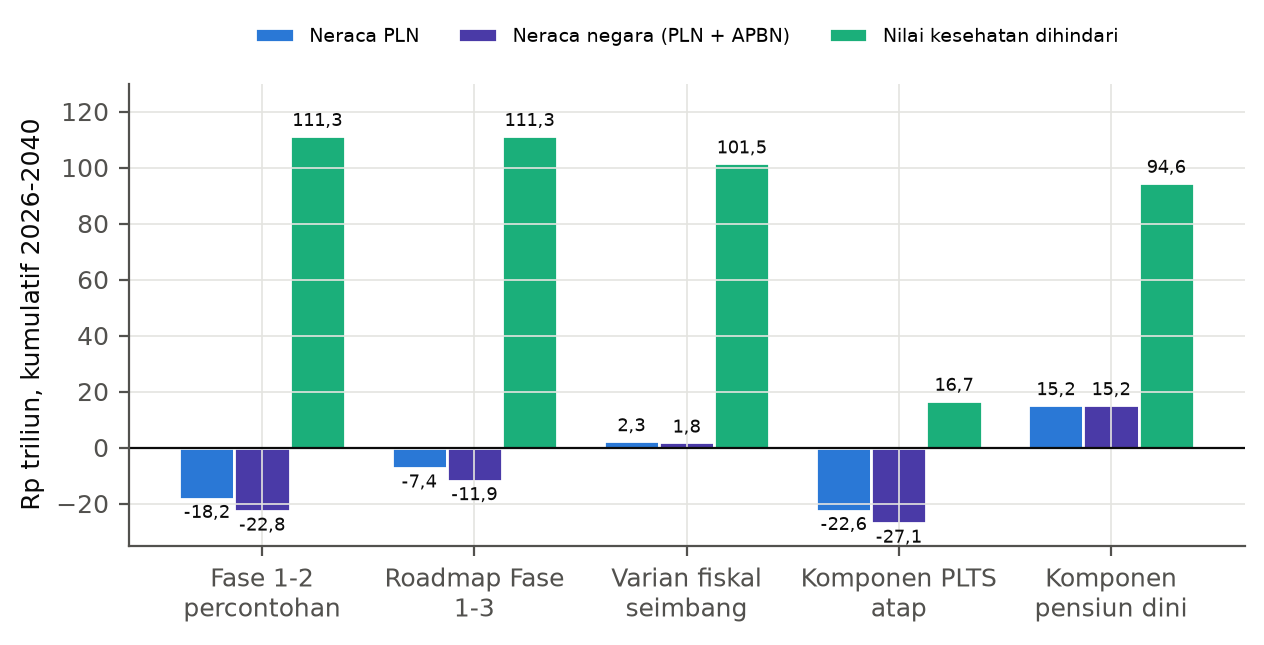
\includegraphics[width=\textwidth]{neraca_preset}
\caption{Neraca PLN, neraca negara, dan nilai kesehatan kumulatif 2026-2040}
\label{fig:neraca}
\sumber{PowerShift, tab Analisis bagian perbandingan skenario}
\end{figure}

Komponen PLTS atap saja membebani negara Rp27,1 triliun karena pendapatan PLN berpindah menjadi hemat tagihan pelanggan. Komponen pensiun dini saja memberi surplus Rp15,2 triliun. Roadmap lengkap menggabungkan keduanya sehingga beban negara turun menjadi Rp11,9 triliun, sementara manfaat kesehatan Rp111,3 triliun dan hemat tagihan pelanggan Rp38,0 triliun tetap diperoleh. Hasil skenario Fase 1-2 menunjukkan hal penting lain. Bila roadmap berhenti setelah percontohan, beban negara naik menjadi Rp22,8 triliun karena PLTS atap terus bertambah tanpa pensiun PLTU IPP berikutnya. Fase 3 karena itu bukan pilihan tambahan, melainkan bagian yang membuat program terjangkau.

\subsection{Biaya dan Skema Pembiayaan}

Tabel~\ref{tab:biaya} merinci arus biaya dan manfaat roadmap lengkap menurut pihak yang menanggung.

\begin{table}[H]
\centering
\caption{Arus biaya dan manfaat Roadmap Fase 1-3, kumulatif 2026-2040}
\label{tab:biaya}
\small
\begin{tabularx}{\textwidth}{L{3.2cm} Y r}
\toprule
Pihak & Pos & Rp triliun \\
\midrule
PLN & Pembayaran kapasitas PLTU IPP yang dihemat & +52,6 \\
 & Biaya energi yang dihemat & +17,9 \\
 & Pendapatan yang berpindah ke pemilik PLTS atap & -38,0 \\
 & Pembangkit pengganti 3.006 MW & -36,1 \\
 & Porsi PLN dari kompensasi (20\%) & -3,8 \\
 & \textbf{Neraca PLN} & \textbf{-7,4} \\
\addlinespace
APBN dan BUMN & Belanja PLTS atap gedung pemerintah dan BUMN & -33,8 \\
 & Tagihan listrik gedung yang dihemat & +32,8 \\
 & Insentif fiskal industri & -3,6 \\
\addlinespace
Negara & \textbf{PLN ditambah pos APBN} & \textbf{-11,9} \\
\addlinespace
Dana luar & Kompensasi pensiun dini (80\%) melalui ETM dan JETP & 15,2 \\
Pelanggan & Hemat tagihan pemilik PLTS atap & +38,0 \\
Masyarakat & Nilai kematian dini yang dihindari & +111,3 \\
\bottomrule
\end{tabularx}
\sumber{PowerShift, tab Neraca dan unduhan CSV}
\end{table}

Kewajiban PLTS atap gedung pemerintah dan BUMN hampir impas bagi APBN dalam horizon kajian dan berlanjut menguntungkan setelah 2040 karena tagihan terus dihemat. Beban negara bersih Rp11,9 triliun setara rata-rata kurang dari Rp1 triliun per tahun, kecil dibanding subsidi listrik sekitar Rp100 triliun per tahun \cite{B-KONTAN-SUBSIDI-2026}. Kebutuhan dana luar Rp15,2 triliun berada di bawah alokasi pensiun dini CIPP JETP yang sekitar US\$1,3 miliar atau Rp21,5 triliun \cite{P-CREA-CIPP-2023}.

\subsection{Proyeksi Dampak dan Capaian Indikator}

Tabel~\ref{tab:kpi} membandingkan hasil model dengan indikator keberhasilan laporan kelompok.

\begin{table}[H]
\centering
\caption{Capaian indikator keberhasilan per skenario}
\label{tab:kpi}
\small
\begin{tabular}{lrrr}
\toprule
Indikator & Fase 1-2 & Roadmap Fase 1-3 & Varian seimbang \\
\midrule
PLTU pensiun dini (GW) & 0,66 & 3,01 & 2,58 \\
Tambahan PLTS atap 2040 (GWp) & 3,19 & 3,19 & 1,30 \\
Rasio PLTS atap terhadap PLTU & 483\% & 106\% & 50\% \\
PLTS atap Jawa-Bali 2028 (MWp) & 1.363 & 1.363 & 1.250 \\
Kuota Jawa-Madura-Bali 2028 (MWp) & 1.850 & 1.850 & 1.850 \\
Dana luar (Rp T) & 6,1 & 15,2 & 13,1 \\
Alokasi pensiun dini CIPP JETP (Rp T) & 21,5 & 21,5 & 21,5 \\
Neraca negara (Rp T) & -22,8 & -11,9 & 1,8 \\
\bottomrule
\end{tabular}

\sumber{PowerShift, tab Indikator roadmap, target dari laporan kelompok \cite{L-LAPORAN-K17}, kuota dari \cite{B-CNBC-ROOFTOP-2028}, dan CIPP JETP \cite{P-CREA-CIPP-2023}}
\end{table}

Roadmap lengkap mencapai indikator kesetaraan. Tambahan PLTS atap 3,19 GWp melampaui 3,01 GW PLTU yang dipensiunkan. Pensiun dini 3,01 GW di Jawa-Bali juga melampaui target JETP nasional 1,7 GW. Kuota PLTS atap 2028 baru tercapai 74\% (1.363 dari 1.850 MWp) karena kewajiban baru berlaku pada 2028. Kuota ini dapat dikejar bila kewajiban gedung pemerintah dan BUMN dimulai pada akhir Fase 1.

Kesetaraan daya tidak sama dengan kesetaraan energi. Faktor kapasitas PLTS atap sekitar 16\%, sedangkan PLTU sekitar 64\%. Gambar~\ref{fig:substitusi} menunjukkan lintasannya per tahun. Selama 2031-2035, tambahan PLTS atap masih tertinggal dari kapasitas PLTU yang sudah pensiun, dengan selisih terbesar sekitar 1,1 GW pada 2035. Mulai 2036, Tanjung Jati B 1-2 dan Cilacap Phase I juga pensiun di baseline sehingga selisih terhadap baseline mengecil, sementara kewajiban dan insentif terus menambah PLTS atap. Tambahan PLTS atap melampaui kapasitas yang pensiun lebih awal sejak 2036 dan mencapai 106\% dari seluruh PLTU yang dipensiunkan pada 2040. Selisih selama Fase 3 ditutup pembangkit pengganti. Dari sisi energi, PLTS atap tambahan mengganti sekitar 31\% energi PLTU yang dipensiunkan. Sisanya dipasok pembangkit pengganti dan armada yang ada. Karena itu, indikator kesetaraan daya sebaiknya dilaporkan bersama indikator energi.

\begin{figure}[H]
\centering
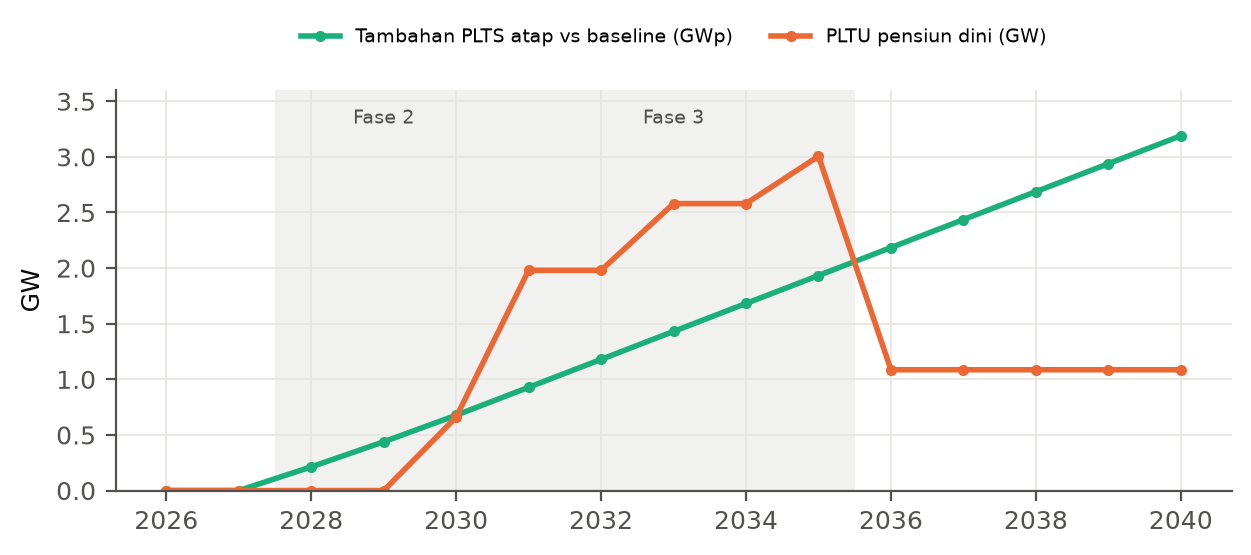
\includegraphics[width=\textwidth]{substitusi_roadmap}
\caption{Tambahan PLTS atap dan kapasitas PLTU pensiun dini per tahun pada Roadmap Fase 1-3}
\label{fig:substitusi}
\sumber{PowerShift, tab Indikator roadmap}
\end{figure}

\subsection{Keandalan Sistem}

\begin{figure}[H]
\centering
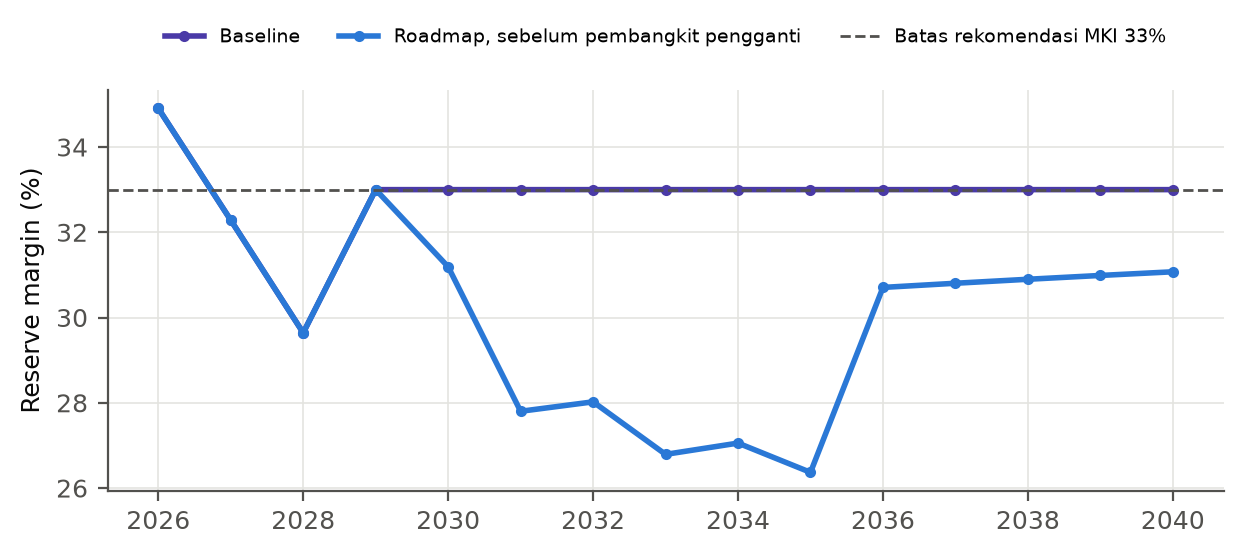
\includegraphics[width=\textwidth]{reserve_margin}
\caption{Reserve margin baseline dan Roadmap Fase 1-3 sebelum pembangkit pengganti}
\label{fig:rm}
\sumber{PowerShift, tab Keandalan, berdasarkan \cite{B-MATAHARI-2024,B-PETROMINDO-RESERVE}}
\end{figure}

Tanpa pembangkit pengganti, reserve margin roadmap turun dari 33\% menjadi 26,4\% pada 2035 (Gambar~\ref{fig:rm}). Kebutuhan pengganti mencapai 3.006 MW pada 2035 dan turun menjadi 1.086 MW setelah 2036 karena sebagian PLTU memang pensiun di baseline. Biaya pengganti sudah dihitung dalam neraca PLN. Rencana tambahan pembangkit Jamali dalam RUPTL 2025-2034 \cite{B-LISTRIKID-RUPTL-JAMALI} dapat dijadwalkan untuk mengisi kebutuhan ini.

\subsection{Sensitivitas}

\begin{figure}[H]
\centering
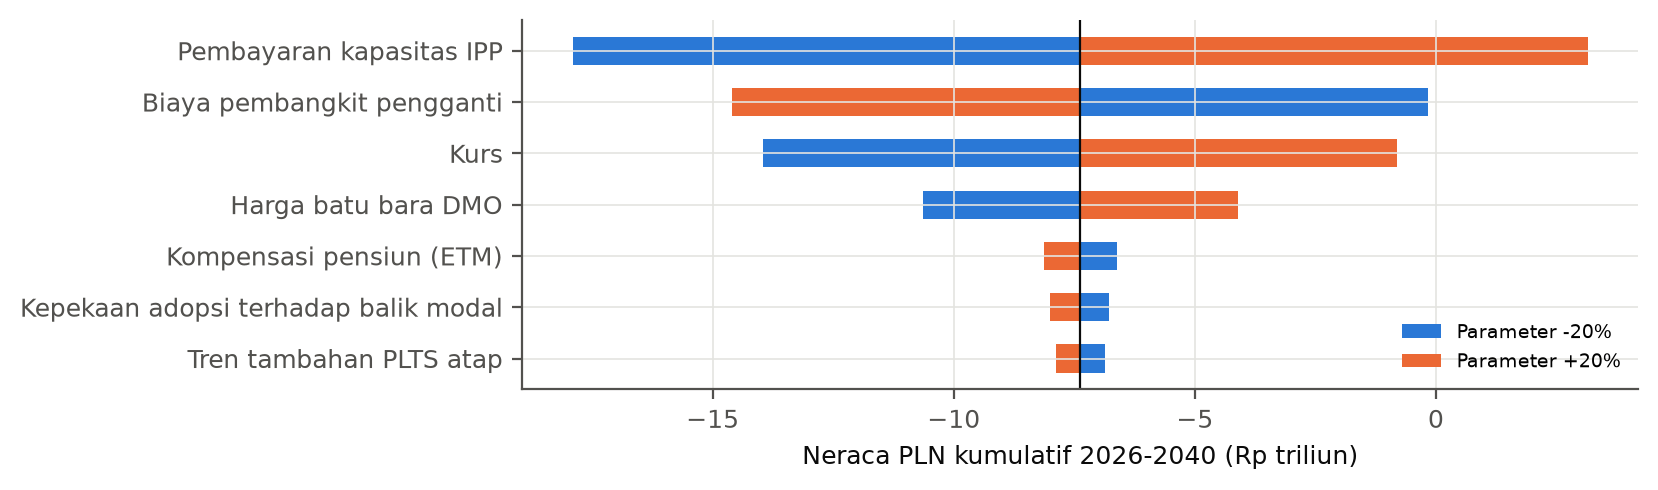
\includegraphics[width=\textwidth]{tornado_roadmap}
\caption{Sensitivitas neraca PLN Roadmap Fase 1-3 terhadap perubahan parameter $\pm$20\%}
\label{fig:tornado}
\sumber{PowerShift, tab Analisis bagian sensitivitas}
\end{figure}

Neraca PLN paling peka terhadap pembayaran kapasitas IPP, biaya pembangkit pengganti, dan kurs (Gambar~\ref{fig:tornado}). Bila pembayaran kapasitas 20\% lebih tinggi dari asumsi, neraca PLN berbalik positif Rp3,1 triliun. Kontrak IPP yang sebenarnya karena itu perlu dimasukkan PLN ke PowerShift sebelum keputusan.

Besaran kompensasi adalah risiko terbesar. Kajian ini memakai estimasi ETM yang dikalibrasi ke refinancing Cirebon-1. Bila kompensasi memakai valuasi ETP yang dirangkum laporan kelompok, beban negara menjadi Rp14,7 triliun dan kebutuhan dana luar Rp26,5 triliun, melampaui alokasi CIPP JETP. Bila memakai klaim PLN untuk Cirebon-1 (Rp60 triliun untuk lima tahun), beban negara menjadi Rp74,3 triliun. Tanpa dana luar sama sekali, beban negara Rp27,1 triliun. Angka-angka ini menegaskan bahwa syarat penutupan K4, yaitu kompensasi yang disepakati dan dana luar yang terikat lebih dulu, menentukan kelayakan program.

\subsection{Risiko dan Mitigasi}

\begin{table}[H]
\centering
\caption{Risiko pelaksanaan dan penanganannya}
\label{tab:risiko}
\small
\begin{tabularx}{\textwidth}{L{3cm} Y Y L{2.4cm}}
\toprule
Risiko & Dampak & Mitigasi & Penanggung jawab \\
\midrule
Klaim kompensasi jauh di atas estimasi & Beban negara dan dana luar membengkak, pensiun dibatalkan & Negosiasi berbasis nilai keuntungan yang hilang, syarat dana terikat sebelum penutupan (K4) & Kemenkeu, PLN \\
\addlinespace
Pembangkit pengganti terlambat & Reserve margin di bawah 33\% & Penutupan ditunda sampai pengganti beroperasi, pengganti masuk RUPTL & PLN, KESDM \\
\addlinespace
Adopsi PLTS atap di bawah target & Indikator kesetaraan tidak tercapai & Kewajiban gedung pemerintah dan BUMN sebagai lantai, insentif industri dinaikkan bila tertinggal & KESDM, Kemenkeu \\
\addlinespace
Integrasi PLTS atap mengganggu jaringan & Tegangan dan frekuensi tidak stabil di siang hari & Penguatan jaringan distribusi dan penyimpanan energi pada Fase 3 & PLN \\
\addlinespace
Pekerja tidak terserap & Penolakan lokal dan ketimpangan baru & Pelatihan ulang dimulai satu tahun sebelum penutupan (K5) & Kemenaker, Pemda \\
\addlinespace
Data kontrak IPP tidak terbuka & Hasil penyaringan meleset & PLN memasukkan data kontrak ke PowerShift secara tertutup, hasil agregat dibuka & PLN, Satgas \\
\bottomrule
\end{tabularx}
\end{table}

\section{Standar Operasional Prosedur dan Kerangka Kelembagaan}
\label{sec:pelaksanaan}

\subsection{Standar Operasional Prosedur Pelaksanaan}

Urutan waktu menentukan keberhasilan program. Pembangkit pengganti membutuhkan beberapa tahun untuk dibangun, sehingga keputusan pensiun dini harus diambil paling lambat tiga tahun sebelum tanggal penutupan. Tabel~\ref{tab:sop} merinci prosedur untuk setiap PLTU kandidat.

\begin{table}[H]
\centering
\caption{SOP pasangan kuota PLTS atap dan pensiun dini per PLTU}
\label{tab:sop}
\small
\begin{tabularx}{\textwidth}{L{2.6cm} Y L{2.6cm} L{2.4cm}}
\toprule
Tahap & Prosedur & Penanggung jawab & Waktu \\
\midrule
1. Penyaringan kandidat & Menjalankan tab Kandidat PLTU di PowerShift dengan data kontrak PLN, mengisi lembar penilaian (Lampiran~\ref{lamp:lembar}), menetapkan daftar urut & Satgas, PLN & Fase 1 (2026-2027), diperbarui tiap tahun \\
\addlinespace
2. Penetapan paket & Menyusun skenario di PowerShift berisi PLTU, tahun pensiun, kuota PLTS atap, dan pendanaan, lalu memeriksa empat syarat penutupan & Satgas, KESDM & $Y-3$ \\
\addlinespace
3. Kesepakatan kompensasi & Negosiasi dengan IPP berbasis keuntungan yang hilang, pengikatan dana luar paling sedikit 80\% & Kemenkeu, PLN, mitra ETM dan JETP & $Y-3$ sampai $Y-2$ \\
\addlinespace
4. Penyiapan pengganti & Menjadwalkan pembangkit pengganti dalam RUPTL dan memulai pembangunan & PLN & $Y-3$ sampai $Y$ \\
\addlinespace
5. Kuota dan kewajiban PLTS atap & Menetapkan kuota sistem, menjalankan kewajiban gedung pemerintah dan BUMN, menyalurkan insentif industri & KESDM, Kemenkeu, Kementerian BUMN & Tahunan sejak 2028 \\
\addlinespace
6. Transisi pekerja & Mendata pekerja, memulai pelatihan ulang dan perlindungan sosial & Kemenaker, Pemda & $Y-1$ \\
\addlinespace
7. Penutupan dan pemantauan & Menutup PLTU setelah syarat terpenuhi, memperbarui skenario di PowerShift dengan realisasi, melaporkan indikator & PLN, Satgas & $Y$ dan tahunan \\
\bottomrule
\end{tabularx}
\sumber{disusun kelompok. $Y$ adalah tahun penutupan PLTU}
\end{table}

\subsection{Kerangka Kelembagaan}

Pembagian peran mengikuti matriks aktor laporan kelompok \cite{L-LAPORAN-K17} dan tata kelola transisi yang dibahas dalam literatur \cite{P-RESOSUDARMO-2023}.

\textbf{Tingkat koordinasi.} Satgas Transisi Energi lintas kementerian menetapkan daftar urut kandidat, memeriksa syarat penutupan, dan meninjau indikator di akhir setiap fase.

\textbf{Tingkat kementerian.} Kementerian ESDM menetapkan kuota berpasangan, kewajiban PLTS atap, dan petunjuk teknis pensiun dini. Kementerian Keuangan mengelola insentif industri, anggaran PLTS atap gedung pemerintah, dan pengikatan dana luar. Kementerian BUMN memastikan kewajiban PLTS atap di gedung BUMN. KLHK mengawasi pemulihan lahan bekas PLTU.

\textbf{Tingkat operator.} PT PLN (Persero) menyusun kajian pensiun dini per PLTU, memasukkan data kontrak ke PowerShift, menyiapkan pembangkit pengganti, dan memperkuat jaringan distribusi untuk PLTS atap.

\textbf{Tingkat daerah dan pendukung.} Kemenaker dan pemerintah daerah menjalankan pelatihan ulang. Sektor swasta dan perbankan membiayai PLTS atap industri. Perguruan tinggi memelihara PowerShift dan memverifikasi parameter sebagai barang publik.

\subsection{Alur Data dan Pelaporan}

Data mengalir berjenjang melalui PowerShift. PLN memasukkan parameter kontrak dan realisasi pembangkitan setiap tahun. KESDM memasukkan realisasi PLTS atap per provinsi. Satgas menjalankan skenario realisasi dan membandingkannya dengan skenario roadmap. Hasil agregat, yaitu neraca per pihak, indikator, dan status syarat penutupan, dibuka kepada publik sebagai tautan skenario, sedangkan data kontrak yang rahasia tetap berada di PLN.

\subsection{Peta Jalan 2026-2040}

\begin{table}[H]
\centering
\caption{Peta jalan roadmap dan keluaran terukur}
\label{tab:fase}
\small
\begin{tabularx}{\textwidth}{L{1.8cm} Y L{4.4cm}}
\toprule
Fase & Langkah utama & Keluaran simulasi akhir fase \\
\midrule
Fase 1 \newline 2026-2027 & Membentuk Satgas, menerbitkan peraturan kuota berpasangan (Lampiran~\ref{lamp:permen}), menetapkan daftar urut kandidat, memulai negosiasi Cirebon-1 & PLTS atap 910 MWp. Belum ada perubahan neraca \\
\addlinespace
Fase 2 \newline 2028-2030 & Kewajiban PLTS atap 200 MW/tahun dan insentif industri 15\% berlaku. Cirebon-1 pensiun 2030 setelah 660 MW pengganti siap & PLTS atap 2.307 MWp. PLTU pensiun 660 MW. Neraca negara -Rp7,4 T. 827 kematian dini dihindari \\
\addlinespace
Fase 3 \newline 2031-2035 & Tanjung Jati B 1-2 pensiun 2031, Cilacap Phase I 2033, Celukan Bawang 2035. Penguatan jaringan dan penyimpanan energi & PLTS atap 4.764 MWp. PLTU pensiun 3.006 MW. Neraca negara -Rp0,6 T. Dana luar Rp10,1 T \\
\addlinespace
Fase 4 \newline 2036-2040 & Evaluasi menyeluruh, penyaringan ulang kandidat termasuk PLTU milik PLN, pemulihan ekonomi daerah & PLTS atap 7.220 MWp. Kumulatif 9.572 kematian dini dan 35,4 Mt CO$_2$ dihindari \\
\bottomrule
\end{tabularx}
\sumber{roadmap laporan kelompok \cite{L-LAPORAN-K17}, keluaran dari simulasi PowerShift}
\end{table}

\section{Kesimpulan dan Rekomendasi}
\label{sec:kesimpulan}

\subsection{Kesimpulan}

PLTS atap dan pensiun dini PLTU belum berjalan bersamaan karena keduanya diatur terpisah, pemilihan PLTU belum menimbang jenis kontrak, kompensasi dan pengganti tidak dipersyaratkan sebelum penutupan, dan tidak ada alat hitung bersama. Program pasangan kuota PLTS atap dan pensiun dini menjawab celah tersebut dengan memasangkan setiap PLTU yang dipensiunkan dengan tambahan PLTS atap setara, mendahulukan PLTU IPP, dan menetapkan syarat penutupan yang jelas.

Pada sistem Jawa-Bali, roadmap Fase 1-3 memensiunkan 3,0 GW PLTU IPP, menambah 3,19 GWp PLTS atap, dan menghindari 9.572 kematian dini serta 35,4 juta ton CO$_2$ selama 2026-2040. Beban negara bersih Rp11,9 triliun, kurang dari Rp1 triliun per tahun, dengan dana luar Rp15,2 triliun yang masih di bawah alokasi CIPP JETP. Pensiun dini PLTU IPP adalah bagian yang membuat program terjangkau, karena PLTS atap tanpa pensiun dini justru membebani negara lebih besar. Kelayakan ini bergantung pada besaran kompensasi, sehingga kesepakatan kompensasi dan pengikatan dana luar harus mendahului keputusan penutupan.

\subsection{Rekomendasi}

\textbf{Kepada Menteri Energi dan Sumber Daya Mineral:}
\begin{enumerate}
  \item Menetapkan peraturan kuota PLTS atap berpasangan dengan rencana pensiun dini (rancangan pada Lampiran~\ref{lamp:permen}) pada Fase 1.
  \item Menambahkan jenis kontrak dan beban kesehatan per lokasi sebagai pertimbangan dalam penilaian kriteria Permen ESDM 10/2025.
  \item Menetapkan kewajiban PLTS atap gedung instansi pemerintah di Jawa-Bali mulai 2028.
\end{enumerate}

\textbf{Kepada Menteri Keuangan:}
\begin{enumerate}[resume]
  \item Menyediakan insentif fiskal 15\% bagi PLTS atap industri dan anggaran PLTS atap gedung pemerintah.
  \item Mensyaratkan pengikatan paling sedikit 80\% kompensasi dari dana luar sebelum keputusan penutupan.
\end{enumerate}

\textbf{Kepada Direktur Utama PT PLN (Persero):}
\begin{enumerate}[resume]
  \item Memasukkan data kontrak IPP ke PowerShift untuk penyaringan kandidat dan membuka hasil agregatnya.
  \item Menjadwalkan pembangkit pengganti dalam RUPTL terhadap tanggal penutupan Cirebon-1, Tanjung Jati B 1-2, Cilacap Phase I, dan Celukan Bawang.
  \item Memperkuat jaringan distribusi Jawa-Bali untuk menyerap 3 GWp PLTS atap tambahan.
\end{enumerate}

\textbf{Kepada Satuan Tugas Transisi Energi:}
\begin{enumerate}[resume]
  \item Memakai PowerShift sebagai alat hitung bersama untuk penetapan daftar urut, pemeriksaan syarat penutupan, dan tinjauan indikator di akhir setiap fase.
  \item Melaporkan indikator kesetaraan daya bersama indikator energi agar substitusi tidak dinilai berlebihan.
\end{enumerate}

\textbf{Kepada Kementerian Ketenagakerjaan dan pemerintah daerah:}
\begin{enumerate}[resume]
  \item Memulai pelatihan ulang pekerja setiap PLTU kandidat paling lambat satu tahun sebelum penutupan, diarahkan ke pemasangan dan pemeliharaan PLTS atap.
\end{enumerate}

Dengan langkah-langkah tersebut, PLTS atap tidak lagi dipandang sebagai pengurang pendapatan PLN, dan pensiun dini tidak lagi dipandang sebagai beban kompensasi semata. Keduanya menjadi satu program yang biayanya terukur dan manfaatnya dapat dibuktikan.


\clearpage
\printbibliography[title={Daftar Pustaka},heading=bibintoc]

\clearpage
\appendix
\renewcommand{\thesection}{\arabic{section}}
\renewcommand{\thesubsection}{\Alph{subsection}}
\titleformat{\section}{\normalfont\large\bfseries}{Lampiran \thesection.}{0.6em}{}
\titleformat{\subsection}{\normalfont\normalsize\bfseries}{\thesubsection.}{0.5em}{}
\addtocontents{toc}{\protect\renewcommand{\protect\cftsecpresnum}{Lampiran }\protect\setlength{\protect\cftsecnumwidth}{6em}}
\section{Rancangan Peraturan Menteri ESDM tentang Kuota PLTS Atap Berpasangan dengan Pensiun Dini PLTU}
\label{lamp:permen}

\begin{center}
\textbf{RANCANGAN}\\
\textbf{PERATURAN MENTERI ENERGI DAN SUMBER DAYA MINERAL}\\
\textbf{REPUBLIK INDONESIA}\\
\textbf{NOMOR \ldots{} TAHUN 2027}\\[4pt]
\textbf{TENTANG}\\[4pt]
\textbf{KUOTA PEMBANGKIT LISTRIK TENAGA SURYA ATAP BERPASANGAN DENGAN PERCEPATAN PENGAKHIRAN WAKTU OPERASI PEMBANGKIT LISTRIK TENAGA UAP}\\[6pt]
DENGAN RAHMAT TUHAN YANG MAHA ESA\\[4pt]
MENTERI ENERGI DAN SUMBER DAYA MINERAL REPUBLIK INDONESIA,
\end{center}

\noindent\textbf{Menimbang:}
\begin{enumerate}[label=\alph*.]
  \item bahwa percepatan pengakhiran waktu operasi PLTU memerlukan sumber energi pengganti dan kepastian pendanaan agar tidak membebani keuangan negara dan keandalan sistem.
  \item bahwa PLTS atap merupakan sumber energi pengganti yang dapat dipasang cepat dengan investasi yang tersebar di sektor publik dan swasta.
  \item bahwa kuota PLTS atap dan percepatan pengakhiran PLTU perlu ditetapkan secara berpasangan agar pengurangan penjualan listrik diimbangi penghematan biaya pembangkitan.
  \item bahwa berdasarkan pertimbangan pada huruf a, huruf b, dan huruf c, perlu menetapkan Peraturan Menteri tentang Kuota PLTS Atap Berpasangan dengan Percepatan Pengakhiran Waktu Operasi PLTU.
\end{enumerate}

\noindent\textbf{Mengingat:}
\begin{enumerate}
  \item Undang-Undang Nomor 30 Tahun 2009 tentang Ketenagalistrikan sebagaimana telah diubah.
  \item Undang-Undang Nomor 16 Tahun 2016 tentang Pengesahan Paris Agreement.
  \item Peraturan Presiden Nomor 112 Tahun 2022 tentang Percepatan Pengembangan Energi Terbarukan untuk Penyediaan Tenaga Listrik.
  \item Peraturan Menteri ESDM Nomor 2 Tahun 2024 tentang PLTS Atap yang Terhubung pada Jaringan Tenaga Listrik.
  \item Peraturan Menteri ESDM Nomor 10 Tahun 2025 tentang Peta Jalan Transisi Energi Sektor Ketenagalistrikan.
\end{enumerate}

\begin{center}\textbf{MEMUTUSKAN:}\end{center}
\noindent Menetapkan: PERATURAN MENTERI ENERGI DAN SUMBER DAYA MINERAL TENTANG KUOTA PLTS ATAP BERPASANGAN DENGAN PERCEPATAN PENGAKHIRAN WAKTU OPERASI PLTU.

\begin{center}\textbf{BAB I KETENTUAN UMUM}\end{center}
\noindent\textbf{Pasal 1.} Dalam Peraturan Menteri ini yang dimaksud dengan:
\begin{enumerate}
  \item Kuota Berpasangan adalah kuota PLTS atap pada suatu sistem yang ditetapkan dengan memperhitungkan kapasitas PLTU yang dijadwalkan mengakhiri operasi lebih awal pada sistem tersebut.
  \item PLTU Kandidat adalah PLTU yang masuk daftar urut percepatan pengakhiran operasi.
  \item Alat Hitung Bersama adalah perangkat perhitungan terbuka yang dipakai untuk menilai dampak usulan terhadap PT PLN (Persero), APBN, pelanggan, keandalan, emisi, dan kesehatan.
\end{enumerate}

\begin{center}\textbf{BAB II KUOTA BERPASANGAN}\end{center}
\noindent\textbf{Pasal 2.} (1) Kuota PLTS atap tahunan pada suatu sistem paling sedikit sama dengan kapasitas PLTU Kandidat yang dijadwalkan berhenti beroperasi pada sistem tersebut dalam tiga tahun berikutnya. (2) Kuota sebagaimana dimaksud pada ayat (1) tidak boleh lebih kecil dari kuota yang telah ditetapkan sebelumnya.

\noindent\textbf{Pasal 3.} (1) Instansi pemerintah dan BUMN wajib memasang PLTS atap pada gedung yang dimiliki atau dikelolanya sesuai target tahunan yang ditetapkan Menteri. (2) Untuk sistem Jawa-Madura-Bali, target sebagaimana dimaksud pada ayat (1) paling sedikit 200 MW per tahun mulai 2028.

\begin{center}\textbf{BAB III DAFTAR URUT DAN SYARAT PENUTUPAN}\end{center}
\noindent\textbf{Pasal 4.} (1) Daftar urut PLTU Kandidat disusun berdasarkan kriteria sebagaimana diatur dalam Peraturan Menteri ESDM Nomor 10 Tahun 2025 dengan tambahan pertimbangan jenis kontrak dan beban kesehatan per lokasi. (2) Penilaian dilakukan dengan Alat Hitung Bersama dan hasil agregatnya diumumkan.

\noindent\textbf{Pasal 5.} PLTU Kandidat dapat diakhiri operasinya apabila: (a) kompensasi telah disepakati dan paling sedikit 80\% pendanaannya telah terikat, (b) pembangkit pengganti telah beroperasi, (c) tambahan PLTS atap kumulatif pada sistem paling sedikit sama dengan kapasitas yang diakhiri, dan (d) program pelatihan ulang pekerja telah berjalan paling sedikit satu tahun.

\begin{center}\textbf{BAB IV PEMANTAUAN}\end{center}
\noindent\textbf{Pasal 6.} (1) Satuan Tugas Transisi Energi meninjau capaian kuota, penutupan, dan indikator transisi pada akhir setiap fase peta jalan. (2) PT PLN (Persero) menyampaikan data realisasi pembangkitan dan parameter kontrak untuk keperluan Alat Hitung Bersama setiap tahun.

\begin{center}\textbf{BAB V KETENTUAN PENUTUP}\end{center}
\noindent\textbf{Pasal 7.} Peraturan Menteri ini mulai berlaku pada tanggal diundangkan.

\section{Lembar Penilaian Kandidat Pensiun Dini}
\label{lamp:lembar}

Lembar ini diisi Satgas untuk setiap PLTU kandidat pada tahap 1 SOP. Angka diambil dari tab Kandidat PLTU, Indikator roadmap, dan Kriteria Permen 10/2025 di PowerShift. Contoh berikut diisi untuk Cirebon-1 dengan tahun pensiun 2030.

\begin{table}[H]
\centering
\small
\begin{tabularx}{\textwidth}{L{5.2cm} Y L{2.6cm}}
\toprule
Isian & Contoh Cirebon-1 & Sumber di PowerShift \\
\midrule
Pemilik dan jenis kontrak & IPP, PPA hingga Juli 2042 & Popup peta \\
Kapasitas dan usia pada tahun pensiun & 660 MW, 18 tahun & Popup peta \\
Tahun pensiun usulan & 2030 & Panel kebijakan \\
Kompensasi (estimasi ETM) & Rp7,6 triliun selama 2030-2040 & Tab Neraca \\
Neraca negara bila dipensiunkan sendiri & +Rp4,3 triliun (+Rp6,5 triliun per GW) & Tab Kandidat PLTU \\
Pembangkit pengganti yang dibutuhkan & 660 MW & Kartu angka \\
Beban kesehatan saat beroperasi & sekitar 910 kematian dini per tahun & Tab Kandidat PLTU \\
Pekerja langsung & sekitar 300 orang & Tab Indikator roadmap \\
Syarat 1: neraca negara per GW $\geq$ 0 & Terpenuhi & Tab Kandidat PLTU \\
Syarat 2: PLTS atap tambahan $\geq$ daya PLTU & Terpenuhi (sekitar 680 MWp pada 2030) & Tab Indikator roadmap \\
Syarat 3: dana luar terikat $\geq$ 80\% & Diisi saat negosiasi & Panel kebijakan \\
Syarat 4: pengganti beroperasi & Diisi saat penutupan & Tab Keandalan \\
Keputusan & Masuk daftar urut Fase 2 & \\
\bottomrule
\end{tabularx}
\end{table}

\noindent Langkah pengisian:
\begin{enumerate}
  \item Buka PowerShift, pilih skenario roadmap, lalu buka tab Kandidat PLTU dan pilih tahun pensiun usulan.
  \item Catat posisi PLTU pada daftar urut, neraca negara, dan beban kesehatannya.
  \item Tambahkan PLTU ke skenario, atur tahun pensiun dan porsi pendanaan di panel kebijakan.
  \item Baca status syarat pada tab Indikator roadmap dan tab Kriteria Permen 10/2025.
  \item Simpan skenario dengan tombol Bagikan dan lampirkan tautannya pada lembar penilaian.
\end{enumerate}

\section{Pemutakhiran Data dari Laporan Kelompok}
\label{lamp:pemutakhiran}

Kajian ini mengutamakan data yang sumbernya dapat diperiksa ulang dan cukup rinci untuk dimodelkan. Tabel berikut mencatat angka laporan kelompok yang dimutakhirkan.

\begin{table}[H]
\centering
\small
\begin{tabularx}{\textwidth}{L{3.6cm} L{3.8cm} Y}
\toprule
Laporan kelompok & Dokumen kajian & Alasan \\
\midrule
Target PLTS atap 2 GW pada 2028 & Kuota 1,85 GW Jawa-Madura-Bali hingga 2028 & Rincian wilayah dari sumber yang sama \cite{B-CNBC-ROOFTOP-2028}, sesuai cakupan kajian \\
\addlinespace
PLTS atap terpasang 772,9 MWp (November 2025) & 538 MWp (Juli 2025) sebagai titik awal model & Angka resmi KESDM yang dapat diperiksa \cite{B-KONTAN-ROOFTOP-2025}, laju tambahan dihitung dari periode yang sama \\
\addlinespace
Harga PLTS atap Rp15-20 juta per kWp (survei 2022) & Rp11-15 juta per kWp per segmen & Harga lebih baru \cite{B-DETIK-HARGA-PLTS} dan dibedakan antara rumah tangga, bisnis, industri, dan gedung pemerintah \\
\addlinespace
Valuasi pensiun dini per PLTU dari ETP & Estimasi ETM yang dikalibrasi ke refinancing Cirebon-1, ETP sebagai uji sensitivitas & Nilai ETP bergantung pada tahun pensiun versi ETP. Refinancing Cirebon-1 US\$250-300 juta adalah transaksi yang terverifikasi \cite{B-REUTERS-CIREBON-2022} \\
\addlinespace
Intensitas emisi rata-rata 790 g CO$_2$/kWh & Faktor emisi per unit PLTU & Dihitung per PLTU dari data GEM \cite{D-GEM-GCPT} \\
\addlinespace
Sekitar 30.000 pekerja sektor batu bara nasional & Pekerja langsung per PLTU yang dipensiunkan & Indikator dibuat per PLTU agar dapat dijadwalkan terhadap tanggal penutupan \cite{B-ECOBUSINESS-CIREBON} \\
\addlinespace
Target pensiun dini 1,7 GW dan alokasi US\$1,3 miliar & Tetap dipakai & Dikonfirmasi tanggapan CREA atas CIPP \cite{P-CREA-CIPP-2023}. Cakupan waktu dana belum pasti sehingga dipakai sebagai pembanding kasar \\
\bottomrule
\end{tabularx}
\end{table}

\section{Parameter Model}
\label{lamp:asumsi}

Status terverifikasi berarti angka dicocokkan ke dokumen asli. Status asumsi berarti pilihan tim kajian yang terdokumentasi. Kode sumber merujuk ke daftar pustaka dan halaman Sumber pada PowerShift.

{\small
\begin{longtable}{p{0.33\textwidth} p{0.2\textwidth} p{0.26\textwidth} p{0.11\textwidth}}
\toprule
Parameter & Nilai & Sumber & Status \\
\midrule
\endhead
Tahun dasar & 2025 tahun & \texttt{-\allowbreak{}} & asumsi \\
Beban puncak tertinggi Jawa-Madura-Bali & 28.077 MW & \texttt{B-\allowbreak{}MATAHARI-\allowbreak{}2024} & terverifikasi \\
Reserve margin Jawa-Madura-Bali 2025 & 0,375 fraksi & \texttt{B-\allowbreak{}PETROMINDO-\allowbreak{}RESERVE} & terverifikasi \\
Pertumbuhan beban dan penjualan & 0,0445 per tahun & \texttt{B-\allowbreak{}PETROMINDO-\allowbreak{}RESERVE} & terverifikasi \\
Tambahan daya mampu 2026-2028 & 1.000 MW/tahun & \texttt{B-\allowbreak{}PETROMINDO-\allowbreak{}RESERVE} & asumsi \\
Batas bawah reserve margin yang direkomendasikan & 0,33 fraksi & \texttt{B-\allowbreak{}PETROMINDO-\allowbreak{}RESERVE} & terverifikasi \\
Penjualan listrik PLN 2025 & 317,69 TWh & \texttt{B-\allowbreak{}CNBC-\allowbreak{}SALES-\allowbreak{}2025} & terverifikasi \\
Porsi penjualan Jawa-Bali & 0,695 fraksi & \texttt{D-\allowbreak{}PLN-\allowbreak{}STAT-\allowbreak{}2025} & terverifikasi \\
Biaya pokok penyediaan 2026 & 1.874 Rp/kWh & \texttt{B-\allowbreak{}KONTAN-\allowbreak{}SUBSIDI-\allowbreak{}2026} & terverifikasi \\
Kurs & 16.500 Rp/US\$ & \texttt{B-\allowbreak{}KONTAN-\allowbreak{}SUBSIDI-\allowbreak{}2026} & terverifikasi \\
Tingkat diskonto NPV & 0,08 per tahun & \texttt{assumption} & asumsi \\
Porsi kerugian PLN yang ditutup APBN & 1 fraksi & \texttt{assumption} & asumsi \\
Mulai tahun PLN menambah pembangkit untuk menjaga target cadangan & 2029 tahun & \texttt{B-\allowbreak{}LISTRIKID-\allowbreak{}RUPTL-\allowbreak{}JAMALI} & asumsi \\
Harga batu bara DMO untuk PLN & 70 US\$/ton & \texttt{B-\allowbreak{}KONTAN-\allowbreak{}DMO-\allowbreak{}2026} & terverifikasi \\
Kalori acuan harga DMO & 6.322 kcal/kg & \texttt{B-\allowbreak{}KONTAN-\allowbreak{}DMO-\allowbreak{}2026} & perlu cek \\
Biaya variabel non bahan bakar PLTU & 50 Rp/kWh & \texttt{assumption} & asumsi \\
Pembayaran kapasitas IPP (komponen A) & 175 US\$/kW/tahun & \texttt{P-\allowbreak{}IEEFA-\allowbreak{}2017} & asumsi \\
Biaya tetap O\&M PLTU milik PLN & 40 US\$/kW/tahun & \texttt{assumption} & asumsi \\
Nilai buku PLTU milik PLN tahun 2022 & 762.000 US\$/MW & \texttt{B-\allowbreak{}PELABUHANRATU-\allowbreak{}VALUASI} & perlu cek \\
Kompensasi pensiun dini, estimasi skema ETM & 1,05 miliar Rp/MW/tahun dipercepat & \texttt{B-\allowbreak{}REUTERS-\allowbreak{}CIREBON-\allowbreak{}2022} & terverifikasi \\
Kompensasi pensiun dini, klaim PLN & 18,18 miliar Rp/MW/tahun dipercepat & \texttt{B-\allowbreak{}PETROMINDO-\allowbreak{}CIREBON-\allowbreak{}BATAL} & terverifikasi \\
Pekerja langsung per MW & 0,4545 orang/MW & \texttt{B-\allowbreak{}ECOBUSINESS-\allowbreak{}CIREBON} & terverifikasi \\
Biaya kapasitas pembangkit pengganti & 120 US\$/kW/tahun & \texttt{assumption} & asumsi \\
Kematian dini rata-rata armada PLTU & 258,6 kematian/GW/tahun & \texttt{P-\allowbreak{}CREA-\allowbreak{}IESR-\allowbreak{}2023} & terverifikasi \\
Biaya kesehatan per kematian & 704.762 US\$/kematian & \texttt{P-\allowbreak{}CREA-\allowbreak{}IESR-\allowbreak{}2023} & terverifikasi \\
PLTS atap terpasang nasional Juli 2025 & 538 MWp & \texttt{B-\allowbreak{}KONTAN-\allowbreak{}ROOFTOP-\allowbreak{}2025} & terverifikasi \\
Porsi PLTS atap di Jawa-Bali & 0,8 fraksi & \texttt{assumption} & asumsi \\
Tambahan PLTS atap Jawa-Bali dengan aturan sekarang & 240 MWp/tahun & \texttt{B-\allowbreak{}KONTAN-\allowbreak{}ROOFTOP-\allowbreak{}2025} & asumsi \\
Kuota PLTS atap Jawa-Bali per tahun & 800 MW/tahun & \texttt{B-\allowbreak{}PVMAG-\allowbreak{}QUOTA} & asumsi \\
Koefisien kurva pangsa pasar vs balik modal & 0,3 1/tahun & \texttt{P-\allowbreak{}NREL-\allowbreak{}SOLARDS} & perlu cek \\
Umur PLTS atap & 25 tahun & \texttt{assumption} & asumsi \\
Lapangan kerja PLTS atap & 24,72 job-year/MW & \texttt{P-\allowbreak{}CEEW-\allowbreak{}2017} & terverifikasi \\
Keluaran puncak AC per kWp & 0,75 fraksi & \texttt{assumption} & asumsi \\
PLTS atap: Rumah tangga non subsidi & Rp15 jt/kWp, pakai sendiri 40\%, tarif Rp1.444,70 & \texttt{B-\allowbreak{}KOMPASTV-\allowbreak{}TARIF-\allowbreak{}2026} & asumsi \\
PLTS atap: Bisnis & Rp13 jt/kWp, pakai sendiri 80\%, tarif Rp1.224,83 & \texttt{D-\allowbreak{}PLN-\allowbreak{}STAT-\allowbreak{}2025} & asumsi \\
PLTS atap: Industri & Rp11 jt/kWp, pakai sendiri 90\%, tarif Rp1.085,39 & \texttt{D-\allowbreak{}PLN-\allowbreak{}STAT-\allowbreak{}2025} & asumsi \\
PLTS atap: Gedung pemerintah & Rp13 jt/kWp, pakai sendiri 80\%, tarif Rp1.583,12 & \texttt{D-\allowbreak{}PLN-\allowbreak{}STAT-\allowbreak{}2025} & asumsi \\
PLTS atap: Program rumah tangga subsidi & Rp12 jt/kWp, pakai sendiri 50\%, tarif Rp605,00 & \texttt{B-\allowbreak{}KOMPASTV-\allowbreak{}TARIF-\allowbreak{}2026} & asumsi \\
Lama respons pasar PLTS atap terhadap perubahan aturan & 4 tahun & \texttt{assumption} & asumsi \\
Subsidi listrik 2026 & 101.170 miliar Rp/tahun & \texttt{B-\allowbreak{}KONTAN-\allowbreak{}SUBSIDI-\allowbreak{}2026} & terverifikasi \\
Pelanggan subsidi 2026 & 44.880.000 pelanggan & \texttt{B-\allowbreak{}KONTAN-\allowbreak{}SUBSIDI-\allowbreak{}2026} & terverifikasi \\
Porsi subsidi di Jawa-Bali & 0,61 fraksi & \texttt{D-\allowbreak{}PLN-\allowbreak{}STAT-\allowbreak{}2025} & asumsi \\
Kuota PLTS atap Jawa-Madura-Bali hingga 2028 & 1.850 MWp & \texttt{B-\allowbreak{}CNBC-\allowbreak{}ROOFTOP-\allowbreak{}2028} & terverifikasi \\
Target pensiun dini nasional hingga 2040 (CIPP JETP) & 1,7 GW & \texttt{P-\allowbreak{}JETP-\allowbreak{}CIPP-\allowbreak{}2023} & terverifikasi \\
Alokasi pensiun dini CIPP JETP & 1,3 miliar US\$ & \texttt{P-\allowbreak{}JETP-\allowbreak{}CIPP-\allowbreak{}2023} & perlu cek \\
Pekerja terdampak tercakup pelatihan ulang atau perlindungan sosial & 1 fraksi & \texttt{L-\allowbreak{}LAPORAN-\allowbreak{}K17} & asumsi \\
\bottomrule
\end{longtable}

}

\section{Hitung Tangan}
\label{lamp:hitung}

Hitung tangan independen (\texttt{validation/cirebon1\_manual.py}) memakai skenario Cirebon-1 pensiun 2035 dengan dorongan PLTS atap dan kompensasi ETM. Seluruh komponen cocok dengan model dengan selisih di bawah 1\%.

\begin{table}[H]
\centering
\small
\begin{tabular}{lrrr}
\toprule
Komponen (Rp T, kecuali disebut) & 2030 & 2035 & 2040 \\
\midrule
Kapasitas PLTS atap (MWp) & 5.937 & 12.525 & 19.112 \\
Pendapatan PLN hilang & -4,80 & -10,54 & -16,29 \\
Kompensasi ekspor PLTS & -2,87 & -6,44 & -10,01 \\
Biaya energi dihemat & 3,03 & 6,75 & 10,55 \\
Pembayaran kapasitas dihemat & 0,00 & 1,91 & 1,91 \\
Porsi PLN kompensasi pensiun & 0,00 & -0,17 & -0,17 \\
Pembangkit pengganti & 0,00 & -1,31 & -1,31 \\
Neraca PLN & -4,64 & -9,80 & -15,32 \\
\bottomrule
\end{tabular}

\end{table}

\section{Daftar Unit PLTU}
\label{lamp:unit}

{\small
\begin{longtable}{p{0.22\textwidth} p{0.15\textwidth} r r l r r}
\toprule
PLTU & Unit & MW & Mulai & Tipe & Pensiun baseline & tCO$_2$/MWh \\
\midrule
\endhead
Adipala & Unit 1 & 660 & 2015 & PLN & 2055 & 0,94 \\
Batang (Central Java Power) & Unit 1 & 950 & 2022 & IPP & 2052 & 0,84 \\
Batang (Central Java Power) & Unit 2 & 950 & 2022 & IPP & 2052 & 0,84 \\
Celukan Bawang & Unit 1 & 142 & 2015 & IPP & 2045 & 1,15 \\
Celukan Bawang & Unit 2 & 142 & 2015 & IPP & 2045 & 1,15 \\
Celukan Bawang & Unit 3 & 142 & 2015 & IPP & 2045 & 1,15 \\
Cilacap Sumber & Phase I Unit 1 & 300 & 2006 & IPP & 2036 & 1,15 \\
Cilacap Sumber & Phase I Unit 2 & 300 & 2006 & IPP & 2036 & 1,15 \\
Cilacap Sumber & Phase II Unit 3 & 660 & 2016 & IPP & 2046 & 0,94 \\
Cilacap Sumber & Phase III Unit 4 & 1.000 & 2019 & IPP & 2049 & 0,84 \\
Cirebon & Unit 1 & 660 & 2012 & IPP & 2042 & 0,94 \\
Cirebon & Unit 2 & 924 & 2023 & IPP & 2053 & 0,84 \\
Indramayu & Unit 1 & 330 & 2010 & PLN & 2050 & 1,06 \\
Indramayu & Unit 2 & 330 & 2011 & PLN & 2051 & 1,06 \\
Indramayu & Unit 3 & 330 & 2011 & PLN & 2051 & 1,06 \\
Jawa-7 & Unit 1 & 991 & 2019 & IPP & 2049 & 0,84 \\
Jawa-7 & Unit 2 & 991 & 2020 & IPP & 2050 & 0,84 \\
Labuan & Unit 1 & 300 & 2009 & PLN & 2049 & 1,06 \\
Labuan & Unit 2 & 300 & 2010 & PLN & 2050 & 1,06 \\
Lontar & Unit 1 & 315 & 2011 & PLN & 2051 & 1,06 \\
Lontar & Unit 2 & 315 & 2012 & PLN & 2052 & 1,06 \\
Lontar & Unit 3 & 315 & 2012 & PLN & 2052 & 1,06 \\
Lontar & Unit 4 & 315 & 2024 & PLN & 2064 & 0,92 \\
Pacitan & Unit 1 & 315 & 2011 & PLN & 2051 & 1,06 \\
Pacitan & Unit 2 & 315 & 2011 & PLN & 2051 & 1,06 \\
Paiton & Unit 1 & 400 & 1994 & PLN & 2030 & 1,19 \\
Paiton & Unit 2 & 400 & 1993 & PLN & 2033 & 1,19 \\
Paiton Baru & Unit 09 & 660 & 2012 & PLN & 2052 & 0,97 \\
Paiton-1 & Unit 7 & 615 & 1999 & IPP & 2029 & 1,06 \\
Paiton-1 & Unit 8 & 615 & 1999 & IPP & 2029 & 1,06 \\
Paiton-2 & Unit 1 & 660 & 2000 & IPP & 2030 & 1,06 \\
Paiton-2 & Unit 2 & 660 & 2000 & IPP & 2030 & 1,06 \\
Paiton-3 & Unit 1 & 815 & 2012 & IPP & 2042 & 0,94 \\
Pelabuhan Ratu & Unit 1 & 350 & 2013 & PLN & 2045 & 1,06 \\
Pelabuhan Ratu & Unit 2 & 350 & 2013 & PLN & 2045 & 1,06 \\
Pelabuhan Ratu & Unit 3 & 350 & 2013 & PLN & 2045 & 1,06 \\
Rembang & Unit 1 & 315 & 2011 & PLN & 2051 & 1,06 \\
Rembang & Unit 2 & 315 & 2011 & PLN & 2051 & 1,06 \\
Serang & Unit 1 & 660 & 2017 & IPP & 2047 & 0,85 \\
Suralaya & Phase I Unit 1 & 400 & 1984 & PLN & 2030 & 1,19 \\
Suralaya & Phase I Unit 2 & 400 & 1985 & PLN & 2030 & 1,19 \\
Suralaya & Phase I Unit 3 & 400 & 1988 & PLN & 2030 & 1,19 \\
Suralaya & Phase I Unit 4 & 400 & 1989 & PLN & 2030 & 1,19 \\
Suralaya & Phase II Unit 1 & 600 & 1996 & PLN & 2036 & 1,10 \\
Suralaya & Phase II Unit 2 & 600 & 1997 & PLN & 2037 & 1,06 \\
Suralaya & Phase II Unit 3 & 600 & 1997 & PLN & 2037 & 1,06 \\
Suralaya & Unit 08 & 625 & 2011 & PLN & 2051 & 0,97 \\
Suralaya & Unit 09 & 1.000 & 2025 & IPP & 2055 & 0,84 \\
Suralaya & Unit 10 & 1.000 & 2025 & IPP & 2055 & 0,84 \\
Tanjung Awar-Awar & Unit 1 & 350 & 2012 & PLN & 2052 & 1,06 \\
Tanjung Awar-Awar & Unit 2 & 350 & 2013 & PLN & 2053 & 1,06 \\
Tanjung Jati B & Unit 1 & 660 & 2006 & IPP & 2036 & 1,04 \\
Tanjung Jati B & Unit 2 & 660 & 2006 & IPP & 2036 & 1,04 \\
Tanjung Jati B & Unit 3 & 660 & 2011 & IPP & 2041 & 0,96 \\
Tanjung Jati B & Unit 4 & 660 & 2012 & IPP & 2042 & 0,96 \\
Tanjung Jati B & Unit 5 & 1.000 & 2022 & IPP & 2047 & 0,84 \\
Tanjung Jati B & Unit 6 & 1.000 & 2022 & IPP & 2047 & 0,84 \\
\bottomrule
\end{longtable}

}


\end{document}
